%--------------------------------------------------------------------------------------------------------------------------
%  YOU MUST PUT THE FILES "gthesis.cls" and  "gct11.clo" IN SAME DIRECTORY
%
%  The content of your thesis goes in "body.tex"
%  Bibtex file in "mybib.bib"
%  If there is an appendix place it in "appendix.tex"
%---------------------------------------------------------------------------------------------------------------------------

\documentclass[11pt,draft]{gthesis}



%---- ADD PACKAGES ------
\usepackage{amssymb}
\usepackage{amsmath}
\usepackage{latexsym}
\usepackage{graphics}
\usepackage{color}
\usepackage{url}
\usepackage{lineno}
\usepackage{verbatim}
\usepackage{tikz}
\usepackage[absolute,overlay]{textpos}
\usepackage{graphicx}
\usepackage{xcolor}
\usepackage{algorithm}
\usepackage{algpseudocode}
\usepackage{subcaption}
\usepackage{titlesec}

\usetikzlibrary{calc,trees,positioning,arrows,fit,shapes,calc}


%Set the depth level to 4
\setcounter{secnumdepth}{4}

%%set the paragraph to subsubsubsection
\titleformat{\paragraph}
{\normalfont\normalsize\bfseries}{\theparagraph}{1em}{}
\titlespacing*{\paragraph}
{0pt}{3.25ex plus 1ex minus .2ex}{1.5ex plus .2ex}



%%for images
\usepackage{caption} % for \captionof



%--- ADD YOUR MACROS ------
\newtheorem{theorem}{Theorem}[section]          % Numbers theorems bysection.
\newtheorem{proposition}[theorem]{Proposition}  % Numbers a proposition by a theorem number.
\newtheorem{lemma}[theorem]{Lemma}             % Numbers a lemma by a theorem number.
\newtheorem{corollary}[theorem]{Corollary}        % Numbers a corollary by a theorem number.
\newtheorem{example}[theorem]{Example}         % Numbers an example by a theorem number.
\newtheorem{examples}[theorem]{Examples}     % Numbers a list of examples by a theorem number.
\newtheorem{remark}[theorem]{Remark}            % Numbers remark by a theorem number.
\newtheorem{remarks}[theorem]{Remarks}         % Numbers a list of remarks by a theorem number.
\newtheorem{conjecture}[theorem]{Conjecture}   % Numbers a conjecture by a theorem number.
\newtheorem{definition}[theorem]{Definition}       % Numbers a definition by a theorem number.

%%Envoironments
\newenvironment{proof}{{\em Proof.}}{\hspace*{\fill}$\Box$\par\vspace{4mm}}

\newcounter{casenum}
\newenvironment{caseof}{\setcounter{casenum}{1}}{\vskip.5\baselineskip}
\newcommand{\case}[2]{\vskip.5\baselineskip\par\noindent {\bfseries Case \arabic{casenum}:} #1\\#2\addtocounter{casenum}{1}}

%%tree 
\tikzset{
  treenode/.style = {shape=rectangle, rounded corners,
                     draw, align=center,
                     top color=white, bottom color=blue!20},
  root/.style     = {treenode, font=\small, bottom color=red!30},
  env/.style      = {treenode, font=\ttfamily\small},
  dummy/.style    = {circle,draw}
}

%------------------------------------------------------------------------------------------------------------------------------------i
\begin{document}

%--- TITLE PAGE   --------------------------
\title{Title of Thesis with all Formula,  \\ Symbols, or Greek Letters Written out in Words }

\author{Patrick Di Salvo}

\type{Thesis}   

\degree{Master of Pokemon, Poke master}     % Change degree/field to PHD if appropriate
\field{Computer Science}  	

%\degree{Doctor of Philosophy} 	
%\field{Computational Sciences}  


\advisorLabel{Advisor}		% set to Advisors if multiple
\advisor{Dr. Sherlock Holmes}
\advisorS{}	        		% if there is a co-advisor, add here

\degreemonth{July}
\degreeyear{2099}

\maketitle

%--- ABSTRACT  --------------------------
% Recommended word limit is 150 for Masters and 350 for doctoral.
% Try to abide.

\begin{abstract}

Present your abstract here.  This template is just an example of an outline to consider for your thesis.  It is a good idea to double-check with the current University's thesis requirements
here:  

\medskip

\small
\centering
 \url{https://www.uoguelph.ca/graduatestudies/current-students/preparation-your-thesis}

\end{abstract}

%============FRONT MATTER=============================
\begin{frontmatter}

%--- ACKNOWLEDGEMENTS  ------

\begin{acknowledgements}

Present your acknowledgements here.

\end{acknowledgements}


%--- TABLE OF CONTENTS AND LIST OF FIGURES  ------

\tableofcontents
\listoftables
\listoffigures

\end{frontmatter}
%======================================================

%--- MAIN BODY OF THESIS  ------
\dsp




%----------------  INTRODUCTION with THESIS STATEMENT ----------------------
\chapter{Introduction}
\label{chapter:intro}

In this chapter we will provide a more comprehensive analysis of the existing research surrounding ladder lotteries. Let {\sc x} be 
a ladder lottery or permutation. 
Throughout this thesis a number of algorithms are presented. Many of these algorithms use the following auxiliary functions: 
\begin{enumerate}
    \item {\sc Print(x)}: Prints {\sc x}.
    \item {\sc Swap(x,y)}: Swaps {\sc x, y}.
    \item {\sc Sort(x)}: Sorts {\sc x} in ascending order.
    \item {\sc Sorted(x)}: Returns true if {\sc x} is sorted in ascending order, else returns false.
    \item {\sc Max(x)}: Returns the maximum element in {\sc x}.
    \item {\sc Min(x)}: Returns the minimum element in {\sc x}.
\end{enumerate}

The study of ladder lotteries as mathematical objects began in 2010, in the paper
Efficient Enumeration of Ladder Lotteries and its Application, written by Matsui, Nakada, Nakano Uehara and Yamanaka~\cite{A1}. 
In this paper the authors present the first algorithm for generating $OptL\{\pi\}$ for some  
arbitrary permutation $\pi$. Since this paper emerged, there have been 
a number of other papers written about ladder lotteries.
These papers include The Ladder Lottery Realization Problem,
Optimal Reconfiguration of Optimal Ladder Lotteries, 
Efficient Enumeration of all Ladder Lotteries with K Bars,
Coding Ladder Lotteries and
Enumeration, Counting, and Random Generation of Ladder Lotteries.
This thesis is also heavily influenced by Efficient Enumeration of Ladder Lotteries and its Application. Throughout Chapter 2, 
we elaborate on the aforementioned papers pertaining to ladder lotteries.




\section{Thesis Statement}
    This thesis provides four full, or partial, solutions to four problems related 
    to ladder-lotteries. The first of these problems is the so called counting problem,, 
    which asks, how many ladders are in $OptL\{\pi\}$? This thesis provides 
    a formula for the exact number of ladders in $OptL\{\pi\}$, for certain 
    cases of $\pi$ as well as a general recurrence relation for $OptL\{\pi\}$
    when $\pi$ is the decending permutation. The second problem is the so called minimum height 
    problem which asks, given all the ladders in $Optl\{\pi\}$, which ladder(s) are 
    the shortest, that is to say which ladders have the smallest height? This thesis 
    provides a theorem as to which ladder(s) in $OptL\{\pi\}$ have the shortest heights.
    The third problem is the so called canonical ladder generation problem. 
    This problem asks, given all permutations of size $N$, is there a Gray Code 
    to generate a canonical ladder from each permutation's $OptL\{\pi\}$? In other words, 
    is there an easy way to transition from one permutation's canonical ladder to the next 
    permutation's canonical ladder until all permutations of size $N$ have had their canonical 
    ladder generated. This thesis provides such a Gray Code. The last problem is the so called encoding problem.
    The encoding problem asks, given a ladder-lottery, provide an optimal compact 
    representation of said ladder-lottery. This thesis provides an encoding for ladder-lotteries.
\section{Overview of Thesis}  

This thesis is broken down into several sections. Firstly, an introuduction to Amidakuji, 
and how they pertain to computer science will be presented. This will be followed by a literature 
review of ladder lotteries in which discussions of solved problems will be 
provided, along with the commonalities between ladder lotteries and 
other mathematical objects. Following the literature review, the methodology
used to conduct the research will be discussed. This section will focus 
primarily on the algorithms used to generate the data for this reasearch. 
Following the methodology section, the findings of the research will be discussed and analyzed. 
In this section there will be proofs and formulas for certain propositions made about ladder 
lotteries. This section will contain the bulk of the findings for this thesis.
Following the results section, a summary of future work will be provided. In this section,
the failures and successes of this research will be analyzed. There will also be commentary on 
open (unsolved) problems related to ladder lotteries and a 
discussion of how research on ladder lotteries could be used in other fields.
Finally, a conlcusion that summarizes the thesis will be provided.

%----------------  BACKGROUND and LITERATURE REVIEW ----------------------
\chapter{Background}
\label{chapter:background}
An interesting property about ladder lotteries is that they can be derived from a 
\emph{permutation} which is a is a unique ordering of objects.
For the purposes on this paper, the objects of a permutation will be integers 
ranging from [$1$ $\dots$ $N$]. \emph{Optimal ladder lotteries} are a special case of ladder 
lotteries in which there is one bar in the ladder for each \emph{inversion} in the permutation.
An \emph{inversion} is a relation between two elements in $\pi$, 
$\pi_{i}$ and $\pi_{j}$, such that if $\pi_{i}>\pi_{j}$ and $i<j$ then $\pi_{i}$ and $\pi_{j}$ 
form an inversion. 
For example, given $\pi=(4,3,5,1,2)$, its iversion set is $Inv(\pi) =\{(4,3),(4,1),(4,2),(3,1),(3,2),(5,1),(5,2)\}$.
Every permutation has a unique, finite set of optimal ladder lotteries associated with it. 
 Thus, the set of optimal ladder lotteries associated with $\pi$, 
 hereby known as \emph{$OptL\{\pi\}$}, is the set containing all ladder lotteries 
 with a number of bars equal to the number if inversions in $\pi$. 
 See Fig. 2.1 for an example of an optimal ladder in $OptL\{(4,3,2,1)\}$.
 For each optimal ladder in $OptL\{\pi\}$, the $N$ 
 elements in $\pi$ are listed at the top of a ladder and each 
 element is given its own line. 
 At the bottom of a ladder is the \emph{sorted permutation}, 
 hereby known as the \emph{identity permutation} \cite{A7}. 
 The  identity permutation of size $N$ is defined as follows - $I:(1, 2, 3, \dots, N)$. 
 Each ladder in $OptL\{\pi\}$ has the minimal number of horizontal bars to sort $\pi$ 
 into the identity permutation. Each bar in a ladder from $OptL\{\pi\}$ uninverts a single 
 inversion in $\pi$ exactly once. For the remainder of this paper, only optimal ladder 
 lotteries will be discussed, with one exception. Therefore when the term ladder lottery is used, assume 
 optimal ladder lottery unless otherwise stated.\par
 
\begin{figure}[!htp]
    \label{fig:ab}
	\begin{minipage}{0.4\textwidth}
		\centering
		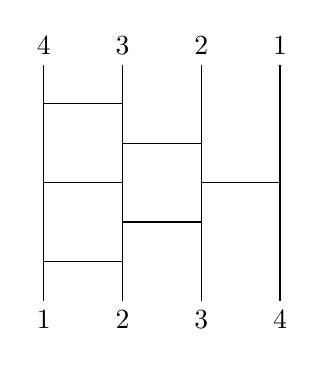
\begin{tikzpicture}
		 	\draw(0, 0) to (0, 3) ++(0, 0) node[above]{4} --(0, 0)node[below]{1};
		 		\draw(0, 2.5) to (1, 2.5);
		 		\draw(0, 1.5) to (1, 1.5);
		 		\draw(0, 0.5) to (1, 0.5);

		 	\draw(1, 0) to (1, 3) ++(0, 0) node[above]{3} --(1, 0)node[below]{2};
		 		\draw(1, 2) to (2, 2);
		 		\draw(1, 1) to (2, 1);
		 	\draw(2, 0) to (2, 3) ++(0, 0) node[above]{2} --(2, 0)node[below]{3};
		 		\draw(2, 1.5) to (3, 1.5);
		 	\draw(3, 0) to (3, 3) ++(0, 0) node[above]{1} --(3, 0) node[below]{4};
		\end{tikzpicture}
				

	\end{minipage}
	\begin{minipage}{.4\textwidth}
		\begin{flushright}
		
		
		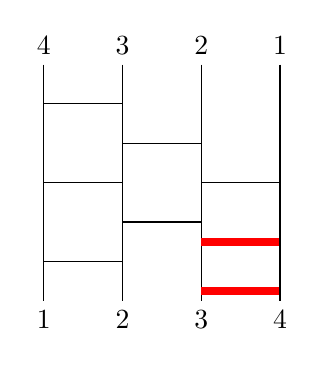
\begin{tikzpicture}
		 	\draw(0, 0) to (0, 3) ++(0, 0) node[above]{4} --(0, 0)node[below]{1};
		 		\draw(0, 2.5) to (1, 2.5);
		 		\draw(0, 1.5) to (1, 1.5);
		 		\draw(0, 0.5) to (1, 0.5);
		 		

		 	\draw(1, 0) to (1, 3) ++(0, 0) node[above]{3} --(1, 0)node[below]{2};
		 		\draw(1, 2) to (2, 2);
		 		\draw(1, 1) to (2, 1);
		 	\draw(2, 0) to (2, 3) ++(0, 0) node[above]{2} --(2, 0)node[below]{3};
		 		\draw(2, 1.5) to (3, 1.5);
		 		\draw[line width=1mm, red](2, 0.75) to (3, 0.75);
		 		\draw[line width=1mm, red](2, 0.125) to (3, 0.125);
		 	\draw(3, 0) to (3, 3) ++(0, 0) node[above]{1} --(3, 0) node[below]{4};
		\end{tikzpicture}
	\end{flushright}
	\end{minipage}
	\caption{Two ladders for the permutation (4, 3, 2, 1). The left ladder is an optimal ladder and the right ladder is not. Therefore the left ladder belongs to $optL\{(4,3,2,1)\}$. The bold  bars in the right ladder are redundant, thus the right ladder is not optimal}
	
\end{figure}


 


\section{Literature Review}
%%Intro to the Literature Review
\subsection{Literature Overview}
    The study of ladder lottieres as mathematical objects began in 2010, in  the paper
    \textbf{Efficient Enumeration of Ladder Lotteries and its Application}. The paper was 
    written by four authors, Yamanaka, Horiyama, Uno and Wasa. In this paper the 
    authors present an algorithm for generating all the ladder lotteries of an 
    arbitrary permutation, $\pi$. Since this paper emerged, there have been 
    several other paper written directly about ladder lotteries. 
    These papers include \textbf{The Ladder Lottery Realization Problem},
    \textbf{Optimal Reconfiguration of Optimal Ladder Lotteries}, 
    \textbf{Efficient Enumeration of all Ladder Lotteries with K Bars},
    \textbf{Coding Ladder Lotteries} and
    \textbf{Enumeration, Counting, and Random Generation of Ladder Lotteries}.

%$input review of first paper
\section{Efficient Enumeration of Laddder Lotteries and its Application}

%%Intro
\subsection{Introduction}
In their paper, \textbf{Efficient Enumeration of Ladder Lotteries and its Application},
the authors provide an algorithm for generating $OptL\{\pi\}$ 
for any $\pi$, in $\mathcal{O}(1)$ per ladder \cite{A1}. This is the first algorithm for generating $OptL\{\pi\}$. 
To see this algorithm please refer to 
Alg.\ref{Alg:FindAllChildren}. The paper also presents the number 
of ladder lotteries in $OptL\{(11, 10, 9, 8, 7, 6, 5, 4, 3, 2, 1)\}$ which is 
$5,449,192,389,984$ \cite{A1}.There are also four other algorithms in 
this section, none of which are found in the paper \emph{Efficient Enumeration of Ladder Lotteries and its Applications}. The 
algorithms are Alg.\ref{Alg:RootLadder}, Alg.\ref{Alg:RightSwap}, Alg.\ref{Alg:LeftSwap} and Alg.\ref{Alg:ShiftChildren}.
These algorithms are used to perform mandatory steps in \ref{Alg:FindAllChildren}. These algorithms are novel.\par 
The authors' algorithm is known as \emph{FindAllChildren}. It is based on several key concepts, the most 
important of which is the \emph{local swap operation}. This is the 
minimal change operation that transitions from one ladder in $OptL\{\pi\}$ to the 
next ladder. The local swap operation is essentially a 180 degree rotation
of three bars in the ladder, such that the bottom
bar is rotated to the top, the middle bar stays in the middle and the top bar
is rotated to the bottom. If the bars undergo a 180 degree rotation to the right, 
then this is known as a \emph{right swap operation} and 
if the bars udergo a 180 degree rotation to the left then this 
is known as a \emph{left swap operation} \cite{A1}. To go to the next ladder in the set, 
the current ladder, $l_{i}$, udergoes a right swap operation 
to get to ladder $l_{i+1}$. See Fig.\ref{fig:rightSwap} for an exmaple of a 
local swap operation. The \emph{route} of an element is the sequence of bars in the ladder that an element must cross 
in order to reach its correct position in 
the identity permutation \cite{A1}. The sequence is ordered from top left to bottom right.
Note, that each bar has two elements that cross it, 
therefore the bar belongs to the route of the greater of the two elements. 
It is important to note that when a right swap operation occurs, 
two of the three bars belong to the route of a unique greater element and one bar belongs
to the route of a unique lesser element. Once rotated, the bar of the lesser element is 
moved above the bars of the greater element.\par
The \emph{clean level} refers to the smallest element 
in $\pi$ such that none of its bars have undergone a right swap operation \cite{A1}.
If there is no such element, then the clean level is the maximum element in $\pi$ + 1.
The \emph{root ladder} is the only ladder in  the set with a clean level of 1; in 
other words, the root ladder is the only ladder in which no bars have undergone 
a right swap operation. The root ladder is unique to $OptL\{\pi\}$. To see the root ladder 
of $OptL\{(4,5,6,3,1,2)\}$ please refer to figure Fig.\ref{fig:root}. The root ladder is
also the \emph{first ancestor  ladder} in $OptL\{\pi\}$. Insofar as the enumeration algorithm 
is based on performing a right swap operation on a pervious ladder, then every other 
ladder in $OptL\{\pi\}$ must have at least one right swap operation. Since the root ladder has
no right swap operations, then it must be an ancestor of every other ladder.\par

%%Root ladder subsection
\subsection{The Root Ladder in Detail}
The authors provide a good description of the root ladder, however they do not provide an algorithm 
for creating the root ladder. Since the root ladder is an ancestor to every other ladder in $OptL\{\pi\}$, 
the root ladder cannot be created using the same algorithm as every other ladder. This thesis provides such 
an algorithm in Alg.\ref{Alg:RootLadder}.\par

\begin{algorithm}
	%%\setstretch{1.35}
	 %% \algsetup{linenosize=\tiny}
	\begin{algorithmic}[1]
		\Function {CreateRoot}{$ladder[2(N-1)-1][N-1]$, $\pi$, $N$, $row \gets 1$}
			\If{$N=1$}
				\State return
			\EndIf
			\State $largestIndex \gets$ index of largest element in $\pi$
			\For{$i \gets largestIndex+1$, $i \leq N$, $i \gets i+1$}
				\If{$\pi_{largestIndex}>\pi_{i}$ $AND$ $largestIndex < i$}
					\State $column \gets i$
					\If{This is the first bar to be added}
						\While{bar cannot be added}
							\State $row \gets row+1$
						\EndWhile
						\State $ladder[row][column] \gets 1$
					\Else 
						\State $row \gets row+1$
						\State $ladder[row][column] \gets 1$
					\EndIf
				\EndIf
			\EndFor
			\State $\pi \gets \pi - largestElement$
			\State $CreateRoot(ladder, \pi, N-1, row \gets 1)$
		\EndFunction

	\end{algorithmic}
	\caption{The algorithm for creating the root ladder of $OptL\{\pi\}$}
	\label{Alg:RootLadder}
\end{algorithm}\pagebreak



Let $ladder$ be a two dimensional array, let $\pi$ be the current state of the permutation, let $N$ be the 
size of $\pi$, let $row$ be the current row in the ladder. First, the index of the largest element in $\pi$ is assigned to $largestIndex$. 
Once found, the algorithm loops from $largestIndex+1$ to $N$. If $\pi_{largestIndex}>\pi_{i}$ then a bar is to be added to 
$ladder$ at $row,column=i$. There are two cases for calculating the $row$. 
\case{\emph{First bar is being added}}{This is the first bar to be added to the route of the largest element. 
$row$ is incremented until a bar can be added to $ladder$ at $row$ 
and $column$. A bar can be added if neither of its endpoints are touching the endpoints of any other bar.}
\case{\emph{Second or greater bar is being added}}{If this is second or greater bar to be added to the route of the 
largest element in $\pi$ then $row \gets row+1$.}
Once all the bars for the route of the largest element have been added, the largest element from $\pi$ is removed, 
$N \gets N-1$ and $row \gets 1$. Then the algorithm makes a recursive call.

\begin{lemma}
	The time complexity for $CreateRoot$ is $O(N^{3})$
\end{lemma}
\begin{proof}
	The outer for-loop of the function runs from some arbitrary index to $N$ on each function call. The inner for loop runs at most 
	$2(N-1)-1$ times which is reduced to $N$. Thus, we get $O(N^{2})$. The following 
	recursion holds, $CreateRoot(N-K) = CreateRoot(N-K+1) + O((N-K)^{2})=CreateRoot(N-K+2) + O((N-K)^{2}) + O((N-K+1)^{2})\dots $. Which is 
	reduced to $O(N(N+1)(2N+1)/6) = O(N^3)$. QED.
\end{proof}
\pagebreak


\begin{figure}[!htp]
	\begin{minipage}{0.4\textwidth}
		\begin{center}

			%%drawing the lines
			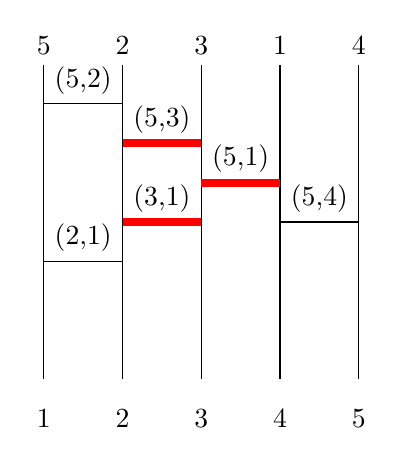
\begin{tikzpicture}
				\draw(0, 0) to (0, 4) node[above]{5};
				\node at (0, -0.5){1};

				\draw(1, 0) to (1, 4) node[above]{2};
				\node at (1, -0.5){2};


				\draw(2, 0) to (2, 4) node[above]{3};
				\node at (2, -0.5){3};

				\draw(3, 0) to (3, 4) node[above]{1};
				\node at (3, -0.5){4};


				\draw(4, 0) to (4, 4) node[above]{4};
				\node at (4, -0.5){5};

				%%drawing the bars

				%%5's route
				\draw(0, 3.5)to (1, 3.5);
					\draw node at (0.5, 3.8) {(5,2)};
				\draw[line width=1mm, red](1, 3) to (2, 3);
					\draw node at (1.5, 3.3) {(5,3)};
				\draw[line width=1mm, red](2, 2.5) to (3, 2.5);
					\draw node at (2.5, 2.8) {(5,1)};
				\draw(3, 2) to (4, 2);
					\draw node at (3.5, 2.3) {(5,4)};

				%%4's route, no bars

				%%3s route
				\draw[line width=1mm, red](1, 2) to (2, 2);
					\draw node at (1.5, 2.3) {(3,1)};
				%%2s route
				\draw(0, 1.5) to (1, 1.5);
					\draw node at (0.5, 1.8){(2,1)};
			\end{tikzpicture}
		\end{center}
	\end{minipage}
	\begin{minipage}{0.4\textwidth}
		\begin{flushright}

			%%drawing the lines
			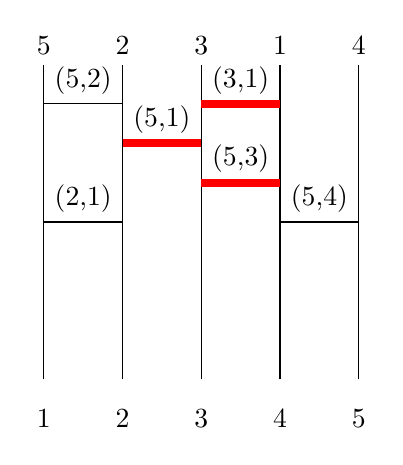
\begin{tikzpicture}
				\draw(0, 0) to (0, 4) node[above]{5};
				\node at (0, -0.5){1};

				\draw(1, 0) to (1, 4) node[above]{2};
				\node at (1, -0.5){2};


				\draw(2, 0) to (2, 4) node[above]{3};
				\node at (2, -0.5){3};

				\draw(3, 0) to (3, 4) node[above]{1};
				\node at (3, -0.5){4};


				\draw(4, 0) to (4, 4) node[above]{4};
				\node at (4, -0.5){5};

				%%Drawing the bars
				\draw(0, 3.5)to (1, 3.5);
					\draw node at (0.5, 3.8){(5,2)};
				\draw[line width=1mm, red](2, 3.5) to (3, 3.5);
					\draw node at (2.5, 3.8) {(3,1)};
				\draw[line width=1mm, red](2, 2.5) to (3, 2.5);
					\draw node at (2.5, 2.8) {(5,3)};
				\draw(3, 2) to (4, 2);
					\draw node at (3.5, 2.3){(5,4)};
				%%4's route, no bars

				%%3s route
				\draw[line width=1mm, red](1, 3) to (2, 3);
					\draw node at (1.5, 3.3) {(5,1)};
				%%2s route
				\draw(0, 2) to (1, 2);
					\draw node at(0.5, 2.3){(2,1)};
			\end{tikzpicture}
		\end{flushright}
	\end{minipage}
	\caption{Example of a local swap operation. When a right swap operation is permformed
	on the left ladder, the result is the right ladder. When a left swap operation is permformed
	on the right ladder, the result is the left ladder.}
	\label{fig:rightSwap}
\end{figure}


\begin{figure}


	\begin{center}
		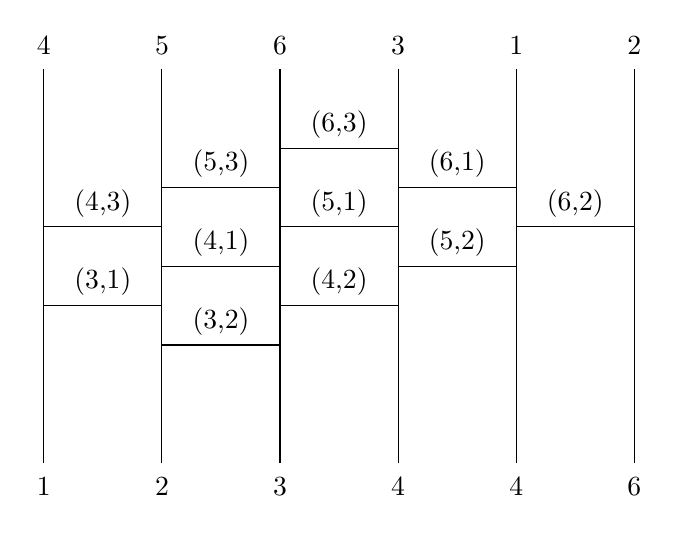
\begin{tikzpicture}
			%%draw the lines
			\draw(0, 0) to (0, 5);
				\node at (0, 5.3){4};
				\node at (0, -0.3){1};

			\draw(1.5, 0) to (1.5, 5);
				\node at (1.5, 5.3){5};
				\node at (1.5, -0.3){2};
			
			\draw(3, 0) to (3, 5);
				\node at (3, 5.3){6};
				\node at (3, -0.3){3};
			\draw(4.5, 0) to (4.5, 5);
				\node at (4.5, 5.3){3};
				\node at (4.5, -0.3){4};
			\draw(6, 0) to (6, 5);
				\node at (6, 5.3){1};
				\node at (6, -0.3){4};
			\draw(7.5, 0) to (7.5, 5);
				\node at (7.5, 5.3){2};
				\node at (7.5, -0.3){6};

			%%draw the bars
			
			%%6's route
			\draw(3, 4) to (4.5, 4);
				\node at (3.75, 4.3){(6,3)};
			\draw(4.5, 3.5) to (6, 3.5);
				\node at (5.25, 3.8){(6,1)};
			\draw(6, 3) to (7.5, 3);
				\node at (6.75, 3.3){(6,2)};
			%%5's route
			\draw(1.5, 3.5) to (3, 3.5);
				\node at (2.25, 3.8){(5,3)};
			\draw(3, 3) to (4.5, 3);
				\node at (3.75, 3.3){(5,1)};
			\draw(4.5, 2.5) to (6, 2.5);
				\node at (5.25, 2.8){(5,2)};
			%draw 4's route
			\draw(0, 3) to (1.5, 3);
				\node at (0.75, 3.3){(4,3)};
			\draw(1.5, 2.5) to (3, 2.5);
				\node at (2.25, 2.8){(4,1)};
			\draw(3, 2) to (4.5, 2);
				\node at (3.75,2.3){(4,2)};

			%%draw 3's route
			\draw(0, 2) to (1.5, 2);
				\node at (0.75, 2.3){(3,1)};
			\draw(1.5, 1.5) to (3, 1.5);
				\node at (2.25, 1.8){(3,2)};
		\end{tikzpicture}

	\end{center}





	\caption{The root ladder for $OptL\{(4,5,6,3,1,2)\}$. Notice how 
	none of the bars have undergone a right swap operation. This is clear 
	when considering that there is no bar of a lesser element above the bar(s)
	of a greater element.} 
	\label{fig:root}

\end{figure}

 %%Save this section for the counting section.
 \begin{theorem}
	 If a ladder from $OptL\{\pi\}$ has not undergone any right swap operations then the ladder is the root ladder. 
	 \label{Theorem:One}
 \end{theorem} 
 \begin{proof}
     The root ladder is defined as the ladder whose clean level is one.
     This means there is no bar of a lesser element above the route a 
     greater element. Keeping in mind that the clean level of the root ladder is one, next consider what is meant by a \emph{child bar}
      which is a bar to the bottom left or right of an arbitrary bar $x$. Within the context of the root ladder, 
      if the left endpoint of the child bar is directly below the right end point of $x$ then the child is a 
     \emph{right child} of $x$. If the right end point of the child bar is directly 
     below the left end point of $x$ then it is a \emph{left child}. Let $x$ belong to the route of element $m$/$Route(m)$.
     If a child is a right child of $x$
	 then it also belongs to the $Route(m)$.
     Let $x$ be a bar representing an inversion with element $m$ and $k$.
     The right child of $x$ is a bar which represents an inversion 
     with $m$ and some element to the right of $k$ termed $k'$. Suppose this was not the case, 
     then this would mean that the right child of $x$ was either a bar representing an inversion 
	 between some element $m'$ such that $m' > m$ or $m' < m$. If $m' > m$ 
	 then this would be a contradiction seeing as $x$ would be above the bar of a route 
     of a greater element which contradicts the definition of the root ladder. On the other hand if 
	 $m' < m$ then $m$ would form an inversion with $m'$ and $x$ would be the bar that uninverted $m$ and $m'$, 
	 but this is also a contradiction seeing as $m' \neq k$ but $x$ uninverts $m$ and $k$. Thus, the right child 
     of $x$ belongs to the same route as $m$ in the root ladder.\par The left child of $x$
     belongs to $Route(l=m-1)$. Suppose this was not the case, 
     then the left child could belong to a route $\geq m$, but if that were the case, this contradicts 
	 the definition of the root ladder seeing as $x$ would be above the route of a greater element. If 
	 $l < m-1$ then the left child of $x$ would be above $Route(m-1)$ which also contradicts the definition 
	 of the root ladder. Therefore, the left child of $x$ must belong to route $l=m-1$. 
	 The second element of the left child of $x$ is $k$. Suppose this was not the case, then 
	 let the second element of the left child be termed $k'$. 
	 $k'$ forms an inversion with $m-1$. But since $m-1 < m$ then $m$ would also form an inversion with $k'$, the 
	 bar corresponding to the inversion $m$ and $k'$ would be $x$. But we already stated that $x$ forms 
	 an inversion between $m$ and $k$, therefore we have another condtradiction. 
	 Therefore, the second element of left child of $x$ must be $k$; the left child of $x$ uninverts elements 
	 $m-1$ and $k$. \par 
	 Please refer to Fig. \ref{Fig:RootChildBars} to view an example of the root ladder for $(3,1,5,2,4)$. Note 
	 that this is a figure of the only ladder in $OptL\{(3,1,5,2,4)\}$.
	 By that the right/left children bars of any given bar 
	 $x$ have not been right swapped, we have proven that if a ladder in $OptL\{\pi\}$ has not undergone 
	 a right swap operation then it must be the root ladder. QED\pagebreak

   
 \end{proof}
 \begin{corollary}
	 If $|OptL\{\pi\}|=1$ then the ladder in $OptL\{pi\}$ must be the root ladder.
 \end{corollary}
 \begin{proof}
	 If there is only one ladder in the set, then that means no bars have been swapped in said ladder. 
	 Thus, it must be the root ladder. QED.
 \end{proof}


 \begin{figure}[!htp]
     \begin{center}
     \begin{tikzpicture}
         \draw(0, 0) to (0, 4);
             \node at(0, 4.3){$3$};
              \draw(0, 3.5) to (2, 3.5);
                 \node at(1, 3.8){$3,1$};
           
             \draw[line width=0.8mm, red](2, 2.5) to (4, 2.5);
                 \node at(3, 2.8){$3,2$};

         \draw(2, 0) to (2, 4);
             \node at(2, 4.3){$1$};
          
         \draw(4, 0) to (4, 4);
              \node at(4, 4.3){5};
                 \draw(4, 3.5) to (6, 3.5);
                     \node at (5, 3.8){$5,2$};
         \draw(6, 0) to (6, 4);
			 \node at(6, 4.3){2};
			 \draw[line width=0.8mm, red](6, 2.5) to (8, 2.5);
			 	\node at(7,2.8){$5,4$};

		\draw(8, 0) to (8, 4);
			\node at(8, 4.3){4};


     \end{tikzpicture}
     \end{center}
     \caption{The root ladder/only ladder in $OptL\{(3,1,5,2,4)\}$ Note that bar 4,2 is the parent of bar 3,2 and 4,1. Also note that 
	 bar 3,2 is the the left child of 4,2 and 4,1 is the right child.}
	 \label{Fig:RootChildBars}
 \end{figure}

%%algorithm
\subsection{$FindAllChildren$}

Let $ladder$ be initilaized as the root ladder. Let $CleanLevel$ be initilaized to $1$. 
Let $N$ be initialized to the max element. The enumeration algorithm 
lists $OptL\{\pi\}$; the authors refer to the algorithm as $FindAllChildren$ \cite{A1}. 
$FindAllChildren$ was used for the bulk of this research, however 
the authors omitted several key steps in the the algorithm. Most notably, they 
omitted the right/left swap operation. Nor do they provide an algorithm 
for permforming a right/left swap operation \cite{A1}. Therefore, I have provided 
the right and left swap operations.
To see $FindAllChildren$ for generating $OptL\{\pi\}$ please refer to Alg.\ref{Alg:FindAllChildren}.
 To see the right/left swap algorithms please 
refer to Alg.\ref{Alg:RightSwap} and Alg.\ref{Alg:LeftSwap} respectively. To 
see an example of a right/left swap operation please refer to Fig.\ref{fig:rightSwap}.
Given an arbitrary bar, $x$, it can be right swapped if and only if there are two bars, $y,z$ where $y \neq z$ 
such that all the following conidtions are met \cite{A1}.
\begin{itemize}
	\item The left end point of $z$ is directly above the left end point of $x$.
	\item The left end point of $y$ is directly above the right end point if $x$.
	\item The right end point of $z$ is directly above the left end point of $y$.
\end{itemize}

Given an arbitrary bar, $x$, it can be left swapped if and only if there are two bars, $y,z$ where $y \neq z$ 
such that the following conditions are met \cite{A1}.
\begin{itemize}
	\item The right end point of $z$ is directly below the right end point of $x$.
	\item The right end point of $y$ is directly below the left end point if $x$.
	\item The left end point of $z$ is directly below the right end point of $y$.
\end{itemize}
In the left ladder in Fig.\ref{fig:rightSwap} bar $x=(3,1)$, bar $y=(5,1)$ and bar $z=(5,3)$. Bar $x$ can be right swapped 
seeing as the three conditions for performing a right swap operation are met.
In the right ladder in Fig.\ref{fig:rightSwap} bar $x=(3,1)$, bar $y=(5,1)$ and bar $z=(5,3)$. Bar $x$ can be left swapped 
seeing as the three conditions for performing a left swap operation are met.


\begin{algorithm}
	\begin{algorithmic}[1]
		\Function{FindAllChildren}{$ladder$, $cleanLevel$, $N$}
			\State $currentRoute \gets N$
			\While{$currentRoute \geq cleanLevel$}
				\State going top left to bottom right 
				\For{$bar \in currentRoute$}
					\State $row \gets$ row of $bar$ in $ladder$ 
					\State $col \gets$ col of $bar$ in $ladder$
					\State $lowerNeighbor \gets ladder[row-1][col]$
					\If{$lowerNeighbor$ is right swappable}
						\State $RightSwap(ladder, bar, lowerNeighbor)$
						\State $FindAllChildren(ladder, y+1, N)$
						\State $leftSwap(ladder, bar, lowerNeighbor)$
					\EndIf
				\EndFor
				\State $currentRoute \gets currentRoute-1$
			\EndWhile
			\State $currentRoute \gets cleanLevel-1$
			\For{$bar \in currentRoute$}
				\State $row \gets$ row of $bar$ in $ladder$ 
				\State $col \gets$ col of $bar$ in $ladder$
				\State $lowerNeighbor \gets ladder[row-1][col]$
				\If{$lowerNeighbor$ is right swappable $AND$ is the rightmost bar of $currentRoute-1$}
					\State $RightSwap(ladder, bar)$
					\State $findAllChildren(ladder, cleanLevel, N)$
					\State $LeftSwap(ladder, bar)$
				\EndIf
			\EndFor
		\EndFunction
	\end{algorithmic}
	\caption{The algorithm for listing $OptL\{\pi\}$.}
	\label{Alg:FindAllChildren}
\end{algorithm}


\begin{algorithm}
	\begin{algorithmic}[1]
		\Function{RightSwap}{$ladder$, $bar$}
			\State $row \gets bar's$ row
			\State $col \gets bar's$ column
			\State $upperNeighbor \gets ladder[row-2][col]$
			\State $rightNeighbor \gets ladder[row-1][col+1]$
			\State $rightSibling \gets ladder[row][col+2]$
			\State $ShiftSubLadder(ladder, rightSibling, 2, 1)$
			\State $Swap(upperNeighbor, ladder[row+1][col+1])$
			\State $Swap(bar, rightNeighbor)$ 
		\EndFunction
	\end{algorithmic}
	\caption{Perform a right swap operation on a bar}
	\label{Alg:RightSwap}
\end{algorithm}
\begin{algorithm}
	\begin{algorithmic}[1]
		\Function{LeftSwap}{$ladder$, $bar$}
			\State $row \gets bar's$ row
			\State $col \gets bar's$ column
			\State $lowerNeighbor \gets ladder[row+2][col]$
			\State $leftNeighbor \gets ladder[row+1][col-1]$
			\State $leftSibling \gets ladder[row][col-2]$
			\State $ShiftSubLadder(ladder, leftSibling, -2, -1)$
			\State $Swap(lowerNeighbor, ladder[row-1][col-1])$
			\State $Swap(bar, leftNeighbor)$
		\EndFunction
	\end{algorithmic}
	\caption{Perform a left swap operation on a bar}
	\label{Alg:LeftSwap}
\end{algorithm}
\begin{algorithm}
	\begin{algorithmic}[1]
		\Function{ShiftSubLadder}{$ladder$, $bar$, $offset$, $index$}
			\If{$ladder[row][col] = 0$}
				\State return
			\EndIf
			\State $row \gets bar's$ row
			\State $col \gets bar's$ column 
			\If{$ladder[row+index][col-index] = 0$ $AND$ $ladder[row+index][col+index] = 0$}
				\State $Swap(ladder[row+offset][col], ladder[row][col])$
			\Else 
				\State $rightChild \gets ladder[row+index][col+index]$
				\State $leftChild \gets ladder[row+index][col-index]$
				\State $ShiftSubLadder(ladder, rightChild, offset, index)$
				\State $ShiftSubLadder(ladder, leftChild, offset, index)$
				\State $Swap(ladder[row+offset][col], Ladder[row][col])$
			\EndIf
		\EndFunction
	\end{algorithmic}
	\caption{Shifts the sub tree of bars up or down the ladder depending on if a right or left swap operation is being performed}
	\label{Alg:ShiftChildren}
\end{algorithm}\pagebreak

The right/left swap functions perform a 180 degree rotation of the bars. When performing a right swap operation, the function 
takes the current bar, $x$, and gets its upper neighbor $z$ and its right neighbor $y$; $x$, $z$ and $y$ meet the 
criteria for performing a right swap operation. The the function calls $ShiftSubLadder$  with the offset value of 
$2$ and the $Index$ value of one. This function ensures that the right sub ladder beginning at the right sibling of $x$, 
located at the same row as $x$ and two columns away from $x$, are shifted down the ladder so that when the right 
swap operation is performed, $z$ will still be above the right sub ladders. To see an example of $RightSwap$ in conjunction with $ShiftSubLadder$ please 
refer to Fig \ref{Fig:SwapAndShift}

\begin{figure}[!htp]
	\begin{minipage}{.4\textwidth}
		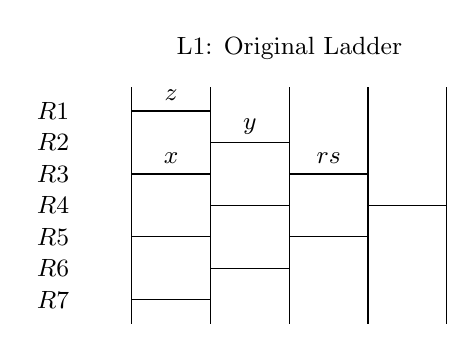
\begin{tikzpicture}
			\node at(2, 3.5){\small{L1: Original Ladder}};
			\draw(0, 0) to (0, 3);
					\node at(.5, 2.9){\small{$z$}};
				\draw(0, 2.7) to (1,2.7);
					\node at(.5, 2.1){\small{$x$}};

				\draw(0,1.9) to (1,1.9);
				\draw(0,1.1) to (1,1.1);
				\draw(0,0.3) to (1,0.3);
			\draw(1, 0) to (1, 3);
				\node at(1.5,2.5){\small{$y$}};
				\draw(1,2.3) to (2,2.3);
				\draw(1,1.5) to (2,1.5);
				\draw(1,0.7) to (2,0.7);
			\draw(2, 0) to (2, 3);
				\node at(2.5, 2.1){\small{$rs$}};
				\draw(2,1.9) to (3,1.9);
				\draw(2,1.1) to (3,1.1);
			\draw(3, 0) to (3, 3);
				\draw(3,1.5) to (4,1.5);
			\draw(4, 0) to (4, 3);

			\node at(-1, 2.7){\small{$R1$}};
			\node at(-1, 2.3){\small{$R2$}};
			\node at(-1, 1.9){\small{$R3$}};
			\node at(-1, 1.5){\small{$R4$}};
			\node at(-1, 1.1){\small{$R5$}};
			\node at(-1, .7){\small{$R6$}};
			\node at(-1, .3){\small{$R7$}};

			
		\end{tikzpicture}
	\end{minipage}
	\begin{minipage}{.4\textwidth}
		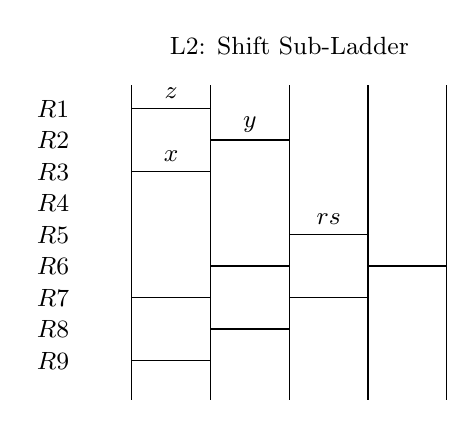
\begin{tikzpicture}
			\node at(2, 3.5){\small{L2: Shift Sub-Ladder}};

			\draw(0, -1) to (0, 3);
					\node at(.5, 2.9){\small{$z$}};
				\draw(0, 2.7) to (1,2.7);
					\node at(.5, 2.1){\small{$x$}};

				\draw(0,1.9) to (1,1.9);
				\draw(0,.3) to (1,.3);
				\draw(0,-0.5) to (1,-0.5);
			\draw(1, -1) to (1, 3);
				\node at(1.5,2.5){\small{$y$}};
				\draw(1,2.3) to (2,2.3);
				\draw(1,0.7) to (2,0.7);
				\draw(1,-0.1) to (2,-0.1);
			\draw(2, -1) to (2, 3);
				\node at(2.5, 1.3){\small{$rs$}};
				\draw(2,1.1) to (3,1.1);
				\draw(2,.3) to (3,.3);
			\draw(3, -1) to (3, 3);
				\draw(3,.7) to (4,.7);
			\draw(4, -1) to (4, 3);

			\node at(-1, 2.7){\small{$R1$}};
			\node at(-1, 2.3){\small{$R2$}};
			\node at(-1, 1.9){\small{$R3$}};
			\node at(-1, 1.5){\small{$R4$}};
			\node at(-1, 1.1){\small{$R5$}};
			\node at(-1, .7){\small{$R6$}};
			\node at(-1, .3){\small{$R7$}};
			\node at(-1, -.1){\small{$R8$}};
			\node at(-1, -.5){\small{$R9$}};


			
		\end{tikzpicture}
	\end{minipage}
		\begin{minipage}{.4\textwidth}
		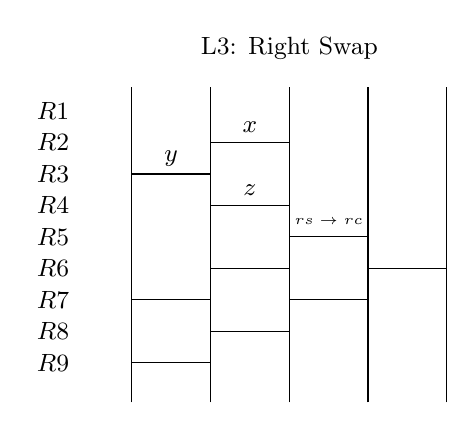
\begin{tikzpicture}
			\node at(2, 3.5){\small{L3: Right Swap}};

			\draw(0, -1) to (0, 3);
					\node at(1.5, 1.7){\small{$z$}};
				
					\node at(.5, 2.1){\small{$y$}};

				\draw(0,1.9) to (1,1.9);
				\draw(0,.3) to (1,.3);
				\draw(0,-0.5) to (1,-0.5);
			\draw(1, -1) to (1, 3);
				\node at(1.5,2.5){\small{$x$}};
				\draw(1,2.3) to (2,2.3);
				\draw(1, 1.5) to (2,1.5);
				\draw(1,0.7) to (2,0.7);
				\draw(1,-0.1) to (2,-0.1);
			\draw(2, -1) to (2, 3);
				\node at(2.5, 1.3){\tiny{$rs \rightarrow rc$}};
				\draw(2,1.1) to (3,1.1);
				\draw(2,.3) to (3,.3);
			\draw(3, -1) to (3, 3);
				\draw(3,.7) to (4,.7);
			\draw(4, -1) to (4, 3);

			\node at(-1, 2.7){\small{$R1$}};
			\node at(-1, 2.3){\small{$R2$}};
			\node at(-1, 1.9){\small{$R3$}};
			\node at(-1, 1.5){\small{$R4$}};
			\node at(-1, 1.1){\small{$R5$}};
			\node at(-1, .7){\small{$R6$}};
			\node at(-1, .3){\small{$R7$}};
			\node at(-1, -.1){\small{$R8$}};
			\node at(-1, -.5){\small{$R9$}};


			
		\end{tikzpicture}
	\end{minipage}
	\caption{$x,y,z$ to be right swapped. $rs$ is the right sibling; the root bar of the right sub-ladder.
	Going right to left, top to bottom. L1=original ladder, L2=shifting the right sub-ladder down two rows. L3 = right swap on $x,y,z$}
	\label{Fig:SwapAndShift}
\end{figure}

When a right swap operation is about to occur, bar $z$ will be moved from its current row and column to its current row + $3$ 
and its current column $+1$. Once the right swap opeartion is performed, 
the right sibling/$rs$ of $x$ becomes the right child/$rc$ of $z$.
The left swap operation is simply the inverse function of the right swap operation. 
Therefore, one can derive the left swap operation and the shift required for left swapping by deriving them 
from the right swap operation and the shift required for the right swap operation.

\begin{lemma}
	Shifting the entire sub-tree beginning at $rs$ down 
two rows ensures that $rs$ becomes $rc(z)$ and the ladder maintains its structure.
\end{lemma}
\begin{proof}
	Assume $ladder$ is a $1$ indexed two dimensional array. Going down the ladder is moving in the positive 
	direction and going up the ladder is moving in a negative direction. 
	Let $k$ be the current row of $z$. Let $k'=k+3$ be the target row of $z$. Let $m$ be the row of $rs$.
	We know that $m$ also equals the row of $x$ seeing as $rs$ is on the same row as $x$ prior to the 
	right swap operation. We know that $k$ = $m-2$ seeing as $z$ is two rows above $x$. Thus, 
	$k'=k+3=(m-2)+3=(m+1)$. Thus, the target row of $z=m+1$. Let $o$ be the current column of $z$.
	Let $o+1$ be the target column of $z$. We know that $o$ is 
	also the column of $x$ seeing as $z$ and $x$ are in the same column. 
	Thus, we know that the column of $rs$ is $o+2$ seeing as $rs$ is the right sibling  
	of $x$. Therefore the target destination of $z$ is $ladder[k'=m+1][o+1]$. 
	$rs$ is in the column $o+2$ and is at $row=m$ prior to the right swap opeartion. 
	We know that $rs \rightarrow rc(z)$ after the right swap operation, therefore $rs$ 
	must appear in the ladder at row $k'+1=m+1+1$ and the column of $o'+1$; please refer to theorem \ref{Theorem:One}
	for the definition of the right child. Since the column of $rs=o'+1$, then the column does not have to be changed.
	Since the current row of $rs$ is $m$, then the right sub-ladder needs to be shfited down by $+2$ to ensure 
	that $rs \rightarrow rc(z)$ after the right swap operation is performed. Since $rs$ also has right and left children, 
	each of them need to be shifted down two rows to ensure the ladder mainatins its structure whence the right swap 
	operation is performed. QED. 

\end{proof}


\pagebreak

%%input revoiew of second paper


\section{Ladder Lottery Realization}

In \emph{Ladder Lottery Realization}~\cite{A3}, written by Horiyama, Uno, Wasa and Yamanaka, the authors provide 
a rather interesting puzzle in regards to ladder lotteries. The puzzle 
is known as the Ladder Lottery Realization Problem. In order to understand
the problem, one must know what a \emph{multi-set} is. A \emph{multi-set}
is a set in which an element may appear more than once. The exponent 
above the element indicates the number of times it appears in the set.
For example, given the following multi-set, $\{3^{2}, 2^{4}, 5^{1}\}$ 
the element $3$ appears twice in the set, the element $2$ appears four times
in the set and the element $5$ appears once in the set.
The Ladder Lottery Realization puzzle asks, given an arbitrary starting permutation, $\pi$, 
and a multi-set of bars, 
is there a ladder lottery for $\pi$
that uses every bar in the multi-set the number 
of times it appears in the  multi-set. 
For an example of an affirmative solution to the Ladder Lottery Realization problem, see Figure~\ref{fig:ladder realization}.

\begin{figure}[!htp]
    \begin{center}
        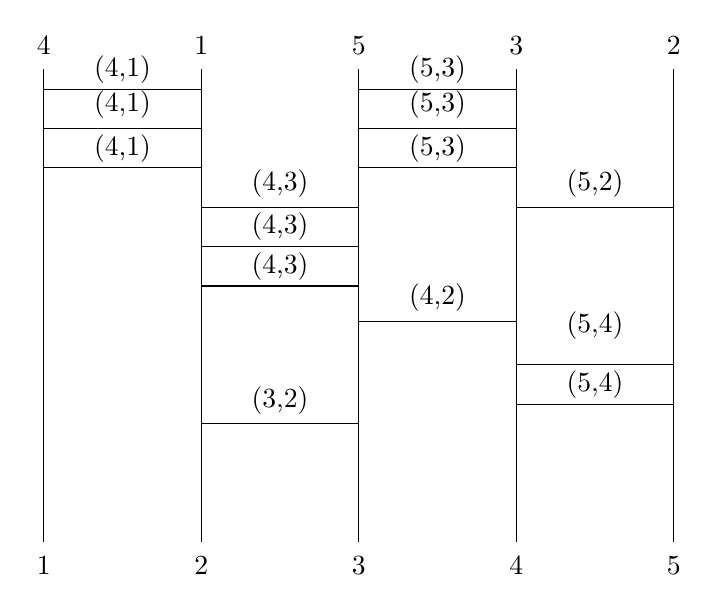
\begin{tikzpicture}
            \draw (0, 0) to (0, 6);
                \node at(0, -0.3){1};
                \node at(0, 6.3){4};
            \draw(2, 0) to (2, 6);
                \node at(2, -0.3){2};
                \node at(2, 6.3){1};
            \draw(4, 0) to (4, 6);
                \node at(4, 6.3){5};
                \node at(4, -0.3){3};
            \draw(6, 0) to (6, 6);
                \node at(6, 6.3){3};
                \node at(6, -0.3){4};
            \draw(8, 0) to (8, 6);
                \node at(8, 6.3){2};
                \node at(8, -0.3){5};

            %%draw the bars
                \node at(1, 6){(4,1)};
                    \draw(0, 5.75) to (2, 5.75);
            \draw(0, 5.25) to (2, 5.25);
                \node at(1, 5.55){(4,1)};
            \draw(0, 4.75) to (2, 4.75);
                \node at(1, 5){(4,1)};

            \draw(4, 5.75) to (6, 5.75);
                \node at(5, 6){(5,3)};
            \draw(4, 5.25) to (6, 5.25);
                \node at(5, 5.55){(5,3)};
            \draw(4, 4.75) to (6, 4.75);
                \node at(5, 5){(5,3)};

            \draw(2, 4.25) to (4, 4.25);
                \node at (3, 4.55){(4,3)};
            \draw(2, 3.75) to (4, 3.75);
                \node at (3, 4){(4,3)};
            \draw(2, 3.25) to (4, 3.25);
                \node at (3, 3.5){(4,3)};
            
            \draw(2, 1.5) to (4, 1.5);
                \node at(3, 1.8){(3,2)};
            
            \draw(4, 2.8) to (6, 2.8);
                \node at (5, 3.1){(4,2)};
            \draw(6, 4.25) to (8, 4.25);
                \node at (7, 4.55){(5,2)};
            
            \draw(6, 2.25) to (8, 2.25);
                \node at (7,2.75){(5,4)};
            
            \draw(6, 1.75) to (8, 1.75);
                \node at (7, 2){(5,4)};
            
        \end{tikzpicture}
    \end{center}
      


    \caption{An affirmative solution to the Ladder Lottery Realization Problem given a starting permutation $(4,1,5,3,2)$ and the multi set of bars $\{(3,2)^{1},(4,1)^{3}, (4,2)^{1},(4,3)^{3},(5,2)^{1},(5,3)^{3},(5,4)^{2}\}$}
    \label{fig:ladder realization}
\end{figure}
\pagebreak
The authors prove that the Ladder Lottery Realization problem in NP-Hard
by reducing the Ladder Lottery Realization to the One-In-Three 3SAT problem, 
which has already been proven to be NP-Hard.
The authors note that there are two cases in which the ladder lottery
realization problem can be solved in polynomial time. These cases 
include the following. First, if every bar in the multi-set appears
exactly once and every bar corresponds to an inversion, 
then an affirmative solution to the Ladder Lottery Realization 
instance can be achieved in polynomial time. 
Second, if there is an inversion in the permutation and its bar appears in the multi-set an even 
number of times, then a negative solution to
the Ladder Lottery Realization instance
can be achieved in polynomial time. This is because the elements that cross the bar will 
be uninverted when then be inverted again. Therefore $\pi$ will not be sorted by the ladder.\par

%%input review of third paper

\section{Optimal Reconfiguration of Optimal Ladder Lotteries}
In Optimal Reconfiguration of Optimal Ladder Lotteries, written by Horiyama, Wasa and Yamanaka,
the authors provide a polynomial solution to the 
\emph{minimal reconfiguration problem} which states that given 
two ladder is $OptL\{\pi\}$, $L_{i}$ and  $L_{m}$, what is the minimal number of 
swap operations to perform that will transition from $L_{i}$ to $L_{m}$~\cite{A2}?
The authors answer the question based on the local swap operations previously 
explained along with some other concepts. The first of these concepts 
is termed the \emph{reverse triple}~\cite{A2}. Basically, a reverse triple is a relation
between three bars, $x,y,z$ in two arbitrary ladders, $L_{i}, L_{m}$, such that if $x,y,x$
are right swapped in $L_{i}$, then they are left swapped in $L_{m}$ or if they are 
left swapped in $L_{i}$ then they are right swapped in $L_{m}$~\cite{A2}. 
The second of the concepts is the \emph{improving triple}~\cite{A2}. The improving triple is 
performing a right/left swapping three bars, $x,y,z$, in $L_{i}$ such that the 
result of the swap removes a reverse triple between
ladders $L_{i}$ and $L_{m}$~\cite{A2}. The improving triple is a symmetric 
relation, therefore performing a right/left swapping of the $x,y,z$ in $L_{m}$ also results in the 
removal of a reverse triple between $L_{i}$ and $L_{m}$~\cite{A2}.\par
The \emph{minimal length reconfiguration sequence} is the minimal number of 
improving triples required to transition from $L_{i}$ to $L_{m}$ or 
$L_{m}$ to $L_{i}$~\cite{A2}. Transitioning from $L_{i}$ to $L_{m}$ with the minimal length reconfiguration sequence 
is achieved by applying an improving triple to each of the reverse triples between 
$L_{i}$ and $L_{m}$. That is to say, the length of the reconfiguration sequence 
is equal to the number of improving triples required to remove all reverse triples between $L_{i}$ and  $L_{m}$~\cite{A2}.\par
The second contribution of this paper is that it provides a closed form formula for the 
upper bound for the minimal length reconfiguration sequence for any permutation 
of size $n$~\cite{A2}. That is to say, given some arbitrary $\pi$ of order $n$, what is the maximum 
length of the minimal length reconfiguration sequence between two ladders in $OptL\{\pi\}$?
The authors prove that there are two unique ladders in $OptL\{\pi=(n, n-1, \dots, 1)\}$ that 
have the upper bound for the minimal length reconfiguration sequence~\cite{A2}. These ladders are the root ladder and \emph{terminating ladder} in 
$OptL\{\pi=(n, n-1, \dots, 1)\}$ that have a minimal reconfiguration sequence equal to 
the upper bound. The terminating ladder in $OptL\{\pi=(n, n-1, \dots, 1)\}$ is defined as the ladder 
such that every possible right swap operation has been performed. The length of the reconfiguration sequence 
between the root ladder and terminating ladder in $OptL\{\pi=(n, n-1, \dots, 1)\}$ is $n{(n-1)~\choose 2}$~\cite{A2}. 
This is because the number of reverse triples between the root ladder and the terminating ladder 
in $OptL\{\pi(n, n-1, \dots, 1)\}$ is equal to $n{(n-1)~\choose 2}$. Thus, in 
order to reconfigure the root to the terminating ladder, or vice versa, each 
reverse triple between them must be improved by applying one improving triple.
\par

%%input review of fourth paper.

\section{Efficient Enumeration of all Ladder Lotteries with K Bars}

In this paper, the authors apply the same algorithm used in Efficient Enumeration of Optimal Ladder-Lotteries 
and its Application for generating all ladder lotteries with k bars. The number of elements 
in The inversion set of $\pi$ also known as $Inv\{\pi\}$ provides the lower bound for $K$ 
and the upper bound is positive infinity. Therefore $K=[|Inv\{\pi\}| \dots N]$\par\par 
\subsection{Coding Latter Lotteries}
\subsubsection{Overview}
In this paper, the authors provide three methods to encode ladder-lotteries as 
binary strings. Coding discrete objects as binary strings is an appealing theme because 
it allows for compact represntation of them for a computer \cite{A5}.
\subsubsection{Route Based Encoding}
The first method is termed \emph{route based encoding method} in 
which each route of an element in the permutation has a binary encoding. Let $L$
be a ladder-lottery for some arbitrary permutation $\pi$ of order $N$. The route 
of element $p_{i}$ is encoded by keeping in mind $p_{i}$ crosses bars in its route 
going left zero or more times and crosses bars in its route going right zero or 
more times \cite{A5}. The maximum number of bars $p_{i}$ can have is $N-1$, therefore the 
upper bound for the number of left/right crossings for $p_{i}$ is $N-1$ \cite{A5}. 
Let a left crossing be denoted with a $'0'$ and let a right crossing be denoted 
with a $'1'$. Let $C_{p_{i}}$ be the route encoding for the $i^{th}$ element 
in $\pi$. To construct $C_{p_{i}}$,  append $0$ and $1$ to each other representing 
the left and right crossings of $p_{i}$ from the top left 
to bottom right of the ladder \cite{A5}. If the number of crossings for $p_{i}$ 
is less than $n-1$, append $0s$ to the encoding of the route of $p_{i}$ until
the encoding is of length $N-1$ \cite{A5}. Let $LC_{L}$ be the route encoding for 
some arbitrary ladder in $OptL\{\pi\}$. $LC_{L}$ is $C_{p_{1}}, C_{p_{2}, \dots C_{p_{N}}}$.
For an example of the route encoding for the root ladder of $(3,2,5,4,1)$ refer to 
Fig.\ref{fig:route-encoding}. In \ref{fig:route-encoding}you will see that $C_{p_{1}}$ is 11\underline{00}. Underlined 
$0s$ are the $0s$ added to ensure the length of $C_{p_{1}}$ is $N-1$.
Since the length of $C_{pi}$ is $N-1$ and the number of elements in $\pi$ is $N$
then the length of $LC_{L}=N(N-1)$. Hence the number of bits needed for $LC_{L}$ 
belongs to $\mathcal{O}(N^{2})$.\par 
\begin{figure}[!htp]
    \begin{center}
        \begin{tikzpicture}
    
            %%draw the lines
            \draw(0, 0) to (0, 4);
                \node at(0, 4.3){3};
                \node at(0, -0.3){1};
            \draw(2, 0) to (2, 4);
                \node at (2, 4.3){2};
                \node at(2, -0.3){2};
            \draw(4, 0) to (4, 4);
                \node at (4, 4.3){5};
                \node at (4, -0.3){3};
            \draw(6, 0) to (6, 4);
                \node at (6, 4.3){4};
                \node at (6, -0.3){4};
            \draw(8, 0) to (8, 4);
                \node at (8, 4.3){1};
                \node at (8, -0.3){5};
    
            %%Draw the bars
            \draw(0, 2) to (2, 2);
            \draw(2, 1.5) to (4,1.5);
            \draw(0, 1) to (2, 1);

            \draw(4, 3) to (6, 3);
            \draw(6, 2.5) to (8, 2.5);
            \draw(4, 2) to (6, 2);
        \end{tikzpicture}
    \end{center}
   
 \caption{The route encoding for the following ladder lottery is 11\underline{00}01\underline{00}11\underline{00}01\underline{00}0000}
 \label{fig:route-encoding}

\end{figure}

\subsubsection{Line Based Encoding}
The second method is termed \emph{line based encoding} which focuses 
on encoding the lines of the ladder-lottery. Each line is represented 
as a sequence of endpoints of bars. Let $L$ be an optimal ladder-lottery 
with $N$ lines and $B$ bars, then for some arbitrary line, $i$, there 
are zero or more right/left endpoints of bars that 
come into contact with $i$ \cite{A5}. Let $LC_{i}$ denote the line based encoding for line $i$.
Let $1$ denote a left end point that 
comes into contact with line $i$ and let $0$ denote a right 
end point that comes into contact with line $i$. Finally, append a $0$
to line $i$ to denote the end of the line. Then line $i$ can be 
encoded, from top to bottom, as a sequence of $1s$ and $0s$ that 
terminates in a $0$.  Given the ladder in Fig. \ref{fig:line-encoding}, 
$LC_{3}$ is $001\underline{0}$. The \underline{0} denotes 
the end of the line. Let $LC_{L}$ be the line encoding for 
some arbitrary ladder, then $LC_{L}=LC_{1}, LC_{2}, \dots LC_{N}$.
Let $L_{(4,2,3,1)}$ refer to the ladder in Fig. \ref{fig:line-encoding}, then 
$LC_{L_{(4,2,3,1)}}=11\underline{0}010\underline{0}110\underline{0}010\underline{0}0\underline{0}$\par 
In order to reconstruct $L$ from its $LC_{L}$, or in other words decode
$LC_{L}$ it is important to recognize that the first line only has left endpoints attached to it
\cite{A5}. Since left end points are encoded as a $1$ then it is guarenteed that the first $0$ 
represents the end of line $1$. Secondly, the last/$Nth$ line 
has only right end points attached to it.  Therefore $LC_{N}$ will only have $0s$. Therefore, $LC_{N}$
does not require a terminating $0$. Thirdly, for any 
line $i+1$, if line $i+1$ has a $0$ then there must be a corresponding $1$
in line $i$. That is to say, if the right end point of a bar is on line 
$i+1$ then that same bar must have a left endpoint on line $i$. To decode 
$LC_{L}$ start by decoding line $1$. The line will contain $0$ or more 
left end points. To decode $LC_{i+1}$ where $i+1>1$, go to 
$LC_{i}$ and match each $1$ in $LC_{i}$ with a $0$ in $LC_{i+1}$. 
Let $k=$ the number of $1s$ in $LC_{i}$. Let $j=$ the number 
of $0s$ in $LC_{i+1}$ then $k=j-1$; due to the last $0$ in $LC_{i+1}$ denoting 
the end of line $i+1$.  Intuitively, this means match every left end point 
of a bar in line $i$ with a right end point in line $i+1$. The last $0$
represents the end of line $i+1$. For an example of a full decoding of $LC_{L_{(4,2,3,1)}}$
please refer to Fig. \ref{fig:line-encoding}.\pagebreak
\begin{figure}[!htp]
    \begin{center}
        \begin{tikzpicture}
            \draw(0, 0) to (0, 4);
            \node at (0, 4.3){4};
            \node at (0, -0.3){1};
        \draw(2, 0) to (2, 4);
            \node at (2, 4.3){2};
            \node at (2, -0.3){2};
        \draw(4, 0) to (4, 4);
            \node at (4, 4.3){3};
            \node at (4, -0.3){3};
        \draw(6, 0) to (6, 4);
            \node at (6, 4.3){1};
            \node at (6, -0.3){4};

        %%bars 
        \draw(0, 3) to (0.7, 3);
            \node at (0.35, 3.3){1};
        \draw (1.3, 3) to (2, 3);
            \node at (1.65, 3.3){0};

        \draw(2, 2.5) to (2.7, 2.5);
            \node at (2.35, 2.8){1};
        \draw(3.3, 2.5) to (4, 2.5);
            \node at (3.65, 2.8){0};

        \draw(4, 2) to (4.7, 2);
            \node at (4.35, 2.3){1};
        \draw(5.3, 2) to (6, 2);
            \node at (5.65, 2.3){0};

      

        \draw(2, 1) to (2.7, 1);
            \node at (2.35, 1.3){1};
        \draw(3.3, 1) to (4, 1);
            \node at (3.65, 1.3){0};

        \draw(0, 0.5) to (0.7, 0.5);
            \node at (0.35, 0.8){1};
        \draw(1.3, 0.5) to (2, 0.5);
            \node at (1.65, 0.8){0};

        \end{tikzpicture}
      

    \end{center}
    \caption{$LC_{L(4,2,3,1)}=LC_{1}=11\underline{0},LC_{2}=0110\underline{0},LC_{3}=010\underline{0},LC_{4}=0$}
    \label{fig:line-encoding}
\end{figure}

Since each bar is encoded as two bits, and there are $N-1$ bits as terminating bits; 
one for each line in $L$, then the number of bits required is $N + 2B -1$, where $N$
is the number of lines and $B$ is the number of bars. Encoding and decoding can be 
done in $\mathcal{O}(n+b)$ time.\cite{A5} Clearly the line-based encoding 
trumps the route-based encoding in both time and space complexity.

\subsubsection{Improved Line-Based Encoding}
Although the line-based encoding is better than the route based 
encoding, it can still be further optimized. The authors provide 
three improvements to the line-based encoding. These three improvements
can be combined to really help imrpove the line based encoding's 
space efficiency \cite{A5}. 
\paragraph{Imrpovement 1}
Since the $Nth$ line has only right endpoints attached to it, 
then it actually does not need to be encoded. Right endpoints 
are denoted as $0$ and left endpoints are encoded as $1$, therefore the number of right endpoints 
for line $N$ is equal to the number of $1s$ in $LC_{N-1}$.
Thus, there is no need for $LC_{N}$ \cite{A5}. The encoding with improvment 
one for the ladder in Fig. \ref{fig:line-encoding} is $11\underline{0}0110\underline{0}010$.
\paragraph{Improvement 2}
Improvement two is based off of the fact that for any two bars,
$x,y$, let $l_{x}$ denote the left endpoint of bar $x$, let 
$l_{y}$ denote the left endoint of bar $y$, let $r_{x}$ denote 
the right end point of bar $x$ and let $r_{y}$ denote the right 
end point of bar $y$. Let line $i$ be the line of $l_{x}$ and $l_{y}$
and let line $i+1$ be the line of $r_{x}$ and $r_{y}$.
\begin{lemma}
There are three possible cases for the 
placement of $x$ and $y$ in some 
arbitrary ladder from $OptL\{\pi\}$. The first case is that there 
is at least one other bar, $z$, with a right end point, $r_{z}$ between $l_{x}$
and $l_{y}$ on line $i$. The second case is that there is at least one other bar 
$z$, with a left end point, $l_{z}$, between $r_{x}$ and $r_{y}$ on line $i+1$. 
The third case is that there is at least one bar, $z$, with a right end point, 
$r_{z}$, betwen $l_{x}$ and $l_{y}$ on line $i$ and there is at least one other bar, 
$z\prime$ with a left end point, $l_{z\prime}$, between $r_{x}$ and $r_{y}$ on line $i+1$ \cite{A5}. 
For an example of all three cases refer to Fig. \ref{fig:three-cases}\par
\end{lemma}

%%figure demonstrating the three cases for bar positions
\begin{figure}[!htp]
       
            %%first case
            \begin{minipage}{.3\textwidth}
                \begin{tikzpicture}
                    \draw(0, 0) to (0, 4);
                        \node at (2, 4.3){\small{$i+1$}};
                    \draw(1, 0) to (1, 4);
                        \node at (1, 4.3){\small{$i$}};
                    \draw(2, 0) to (2, 4);
                        \node at (0, 4.3){\small{$i-1$}};
                    \draw(0, 2) to (1, 2);
                        \node at (.5, 2.3){\small{$r_{z}$}};
                    \draw(1, 3) to (2, 3);
                        \node at (1.5, 3.3){\small{$l_{x}$}};
                    \draw(1, 1) to (2, 1);
                        \node at (1.5, 1.3){\small{$l_{y}$}};
                \end{tikzpicture}
            \end{minipage}
              \begin{minipage}{.3\textwidth}

                 \begin{tikzpicture}
                
                  \draw(0, 0) to (0, 4);
                     \node at (0, 4.3){\small{$i-1$}};
                  \draw(1, 0) to (1, 4);
                    \node at (1, 4.3){\small{$i$}};
                  \draw(2, 0) to (2, 4);
                     \node at (2, 4.3){\small{$i+1$}};
                   \draw(0, 3) to (1, 3);
                         \node at (.5, 3.3){\small{$r_{x}$}};
                    \draw(1, 2) to (2, 2);
                         \node at (1.5, 2.3){\small{$l_{z}$}};
                     \draw(0, 1) to (1, 1);
                         \node at (0.5, 1.3){\small{$r_{y}$}};
                
                   
                
                \end{tikzpicture}
             \end{minipage}
             \begin{minipage}{.3\textwidth}

                \begin{tikzpicture}
                
                 \draw(0, 0) to (0, 4);
                    \node at (1, 4.3){\small{$i$}};
                 \draw(1, 0) to (1, 4);
                    \node at (2, 4.3){\small{$i+1$}};
                 \draw(2, 0) to (2, 4);
                    \node at (0, 4.3){\small{$i-1$}};
                 \draw(3, 0) to (3, 4);
                    \node at (3, 4.3){\small{$i+2$}};
                    \draw(1, 3) to (2, 3);
                        \node at (1.3, 3.3){\small{$l_{x}$}};
                        \node at (1.7, 3.3){\small{$r_{x}$}};
                     \draw(0, 2) to (1, 2);
                        \node at (0.7, 2.3){\small{$r_{z}$}};
                    \draw(1, 1) to (2, 1);
                        \node at (1.3, 1.3){\small{$l_{y}$}};
                         \node at (1.7, 1.3){\small{$r_{y}$}};
                     \draw(2, 2) to (3, 2);
                        \node at (2.3, 2.3){\small{$l_{z\prime}$}};
                
                   
                
                \end{tikzpicture}
            \end{minipage}
        

    \caption{Three examples of the three cases for the placement 
    of bars $x$ and $y$ in a ladder-lottery}
    \label{fig:three-cases}
\end{figure}
\begin{proof}
    Suppose that none of the above cases hold. Let $L_{\pi}$ be an 
    optimal ladder-lottery with bars $x$ and 
    bar $y$. If none of the cases hold then $x$ and $y$ are directly above/below each other without 
    the enpoint of some third bar $z$ between $l_{x}$ and $l_{y}$ or between $r_{x}$ and $r_{y}$.
    Let $x$ be the bar for the inversion of two elements $p$ and $q$ in $\pi$. 
    As $p$ and $q$ travel through the ladder they will cross each other at bar $x$; 
    thus uninverting them. Since bar $y$ is directly below bar $x$, then $p$ and $q$ will cross 
    bar $y$ thus re-inverting them. Therefore, there will need to be a third 
    bar that uninverts $p$ and $q$ a second time. Since this third bar is 
    redundant, $L_{\pi}$ is non-optimal which is a contradiction. Let $x$ be a bar for two 
    elements in $\pi$, $p$ and $q$ such that $p$ and $q$ do not form an inversion. Then $x$ 
    will invert $p$ and $q$ and $y$ will uninvert them. Thus making both $x$ and $y$ redundant
    bars which is also a contradiction. Therefore one of the above cases must hold.
\end{proof}
Knowing that one of the three above cases must hold is beneficial for improving the 
line-based encoding. If $l_{x}$ and $l_{y}$ on line $i$ have no $r_{z}$ between them, 
then there must be at least one $l_{z\prime}$ between $r_{x}$ and $r_{y}$ on line $i+1$.
Since a left endpoint is encoded as a $1$ and a right endpoint is encoded as a $0$, 
a $1$ can be omitted for the encoding of line $i+1$ if $l_{x}$ and $l_{y}$ have no $r_{z}$
between them on line $i$ \cite{A5}. That is to say, if there is not a $0$ between 
the two  $1s$ for $l_{x}$, $l_{y}$ in $LC_{i}$, it is implied that there is at least one $1$ between 
the two $0s$ for $r_{x}$, $r_{y}$ on $LC_{i+1}$. Hence, one of the $1s$ in $LC_{i+1}$ can be omitted. 
The line encoding with improvement two for the ladder in Fig. \ref{fig:line-encoding} is $11\underline{0}010\underline{0}00\underline{0}0$.
\paragraph{Imrpovement 3}
Improvement three is based off of saving some bits for right 
end points/$0s$ in $LC_{N-1}$. Since line $N$ has no left end points,
then then there must be some right endpoints between any two 
consecutive bars connecting lines $N-1$ and line $N$. If you 
refer to Fig. \ref{fig:improvement3}, then the only configuration for lines $N-2, N-1, N$
is the middle configuration \cite{A5}. Knowing this, then 
given two bars, $x$ and $y$ with $l_{x}$/$l_{y}$ on line 
$n-1$ and $r_{x}$/$r_{y}$ on line $n$, there must be at least 
one bar, $z$, with its $r_{z}$ between $l_{x}$ and $l_{y}$
on line $N-1$. Thus, for every $1$ in $LC_{N-1}$ except the 
last $1$ in $LC_{N-1}$, a $0$ must immidediately proceed any $1$
in $LC_{N-1}$. Since this $0$ is implied, it can be removed from $LC_{N-1}$ \cite{A5}. 
For an example of improvement three with its line encoding for $LC_{N-1}$ please refer to Fig.\ref{fig:improvement3}\pagebreak
\begin{figure}[!htp]
    \centering
    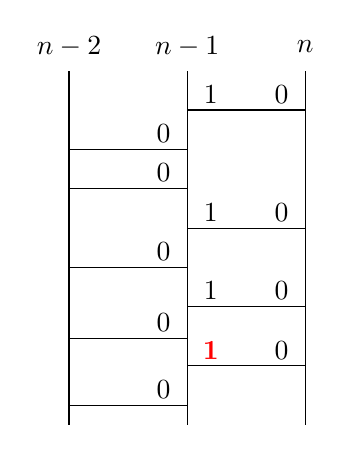
\begin{tikzpicture}
        \draw(0, -0.5) to (0, 4);
            \node at (0, 4.3){$n-2$};
            \draw(0, 3) to (1.5, 3);
                \node at (1.2, 3.2){$0$};
            \draw(0, 2.5) to (1.5, 2.5);
                \node at (1.2, 2.7){$0$};
            \draw(0, 1.5) to (1.5, 1.5);
                \node at (1.2, 1.7){$0$};
            \draw(0, 0.6) to (1.5, 0.6);
                 \node at (1.2, 0.8){$0$};
            \draw(0, -0.25) to (1.5, -0.25);
                \node at (1.2, -0.05){$0$};
        \draw(1.5, -0.5) to (1.5, 4);
            \node at (1.5, 4.3){$n-1$};
            \draw(1.5, 3.5) to (3, 3.5);
                \node at (1.8, 3.7){$1$};
                \node at (2.7, 3.7){$0$};
            \draw(1.5, 2) to (3, 2);
                \node at (1.8, 2.2){$1$};
                \node at (2.7, 2.2){$0$};
            \draw(1.5, 1) to (3, 1);
                \node at (1.8, 1.2){$1$};
                \node at (2.7, 1.2){$0$};
            \draw(1.5, 0.25) to (3, 0.25);
                \node at (1.8, 0.45){$\textcolor{red}{\textbf{1}}$};
                \node at (2.7, 0.45){$0$};

        \draw(3, -0.5) to (3, 4);
            \node at (3, 4.3){$n$};
    \end{tikzpicture}
    \caption{The line coding for $LC_{N-1}$ with imrpovement three is $101110$\underline{$0$}. The red, bold $1$ represents 
    the last left end point in $LC_{N-1}$, therefore the proceeding $0$ must be 
    included in $LC_{N-1}$. For every other $1$ in $LC_{N-1}$, a $0$ is omitted following 
    said $1$.}
    \label{fig:improvement3}
\end{figure}
\paragraph{Combining All Three}
The combination of all three improvements can be done independently. 
Let $IC_{L_{(4,2,3,1)}}$ be the \emph{improved line-based encoding} for $L_{(4,2,3,1)}$ 
by applying improvements 1-3 to $LC_{L_{(4,2,3,1)}}$. Recall that $LC_{L}$ denotes the line-based encoding for some ladder $L$.
$LC_{L_{(4,2,3,1)}}$ for the ladder in Fig. \ref{fig:line-encoding} is $11\underline{0}10101\underline{0}0010101\underline{0}000$.
By applying imrpovement one, we get $11\underline{0}101011\underline{0}0010101\underline{0}$. 
Notice how the last three $0s$ from $LC_{L}$ were removed because they represented $LC_{N}$.
By applying imrpovement two to improvememt one we get $11\underline{0}10011\underline{0}001001\underline{0}$.
Notice how the second, and eigth $1$ were removed because they are implied by 
the successive $0s$. By applying improvement three to the result of improvement 
two we get $11\underline{0}10011\underline{0}00101\underline{0}$. Notice how the last $0$ 
was removed from improvement two. This is because the $0$ is implied in $LC_{N-1}$
due to the configuration between of bars connecting lines $N-1$ and line $N$. The $IC_{L_{(4,2,3,1)}}$ for the ladder in fig. \ref{Fig:allthree} 
is $IC_{L_{(4,2,3,1)}}=11\underline{0}10011\underline{0}00101\underline{0}$.\pagebreak

\begin{figure}[!htp]
     \centering
    \begin{tikzpicture}
         \draw(0, 0) to (0, 4);
             \node at (0, 4.3){$n-3$};
             \draw(0, 3.5) to (1.5, 3.5);
             \draw(0, 2.5) to (1.5, 2.5);
         \draw(1.5, 0) to (1.5, 4);
             \node at (1.5, 4.3){$n-2$};
             \draw(1.5, 3) to (3, 3);
             \draw(1.5, 3.8) to (3, 3.8);
             \draw(1.5, 2) to (3, 2);
             \draw(1.5, 1) to (3, 1);
         \draw(3, 0) to (3, 4);
             \node at(3, 4.3){$n-1$};
             \draw(3, 2.5) to (4.5, 2.5);
             \draw(3, 1.5) to (4.5, 1.5);
             \draw(3, 0.5) to (4.5, 0.5);
         \draw(4.5, 0) to (4.5, 4);
             \node at(4.5, 4.3){$n$};
     \end{tikzpicture}
     \caption{A ladder used to illustrate all three improvements $IC_{L}$. $IC_{L}=11\underline{0}10011\underline{0}00101\underline{0}$}
     \label{Fig:allthree}
\end{figure}

%%%section on how ladde lotteries relate to other mathematical objects
% Despite the fact that ladder lotteries have only been stuidied in and
% of themseleves for ten years, they are closely tied to other mathematical 
% phenomena that have been studied for much longer. These mathematical phenomena  
%  include \emph{Pseudo Lines} which are an arrangement of 
% curves on a plane such that given two curves, they only intersect 
% at most once and at each intersection, only two curves intersect.See figure --reference--
% for a wiring diagrams of the pseudo line arrangement for the 
% permutation, $(5,4,3,2,1)$. The other mathematical phenomena is \emph{adjacent transpositions}
% which is a swap of two adjacent elements in a permutation. 
\subsection{Ladders and Adjacent Transpositions}
A ladder lottery is a way of sorting a permutation, yet it can also be thought of as 
a decomposition of a permutation into \emph{adjacent transpositions}. \cite{A1} 
An \emph{adjacent transposition} is simply a swap of two adjacent elements in a 
permutation. For example, given the permutation (1, 3, 4, 2), an adjacent 
transposition could be done on the following pairs of elements: 
(1, 3), (3, 4) or (4, 2). Each would result in a unique permutation. 
Simply put, given any arbitrary starting permutation, $\pi$, keep swapping 
adjacent inversions until the identity permutation is reached.  An optimal 
ladder lottery from $\pi's$ optimal ladder set is a minimal sequence of 
adjacent transpositions such that $\pi$ is sorted into the identity permutation; 
each ladder in the set represents a sequence of adjacent transpositions for 
sorting $\pi$ into the identity permutation. For example, given the permutation 
(4, 3, 2, 1) there exists eight ladders in this permutation's optimal ladder set. 
Two of these ladders are found in \ref{fig:ac}:

\begin{figure}[!htp]
    \label{fig:ac}
	\begin{minipage}{0.4\textwidth}
		\centering
	
		\begin{tikzpicture}
			\draw(0, 0) to (0, 4) node[above]{4};
			\draw(2, 0) to (2, 4) node[above]{3};
			\draw(4, 0) to (4, 4) node[above]{2};
			\draw(6, 0) to (6, 4) node[above]{1};
			
			\draw(0, 3.7) to (2, 3.7);
				\draw node at (1, 3.9) {(4, 3)};
			\draw(2, 3.25) to (4, 3.25);
				\draw node at (3, 3.45){(4, 2)};
			\draw(4, 2.75) to (6, 2.75);
				\draw node at (5, 3.0){(4, 1)};
			
			\draw(0, 2.75) to (2, 2.75);
				\draw node at (1, 3.0){(3, 2)};
			\draw(2, 2.25) to (4, 2.25);
				\draw node at (3, 2.5){(3, 1)};
			
			
			\draw(0, 1.75) to (2, 1.75);
				\draw node at (1, 1.95){(2, 1)};
			
			\draw node at (0, -0.5){1};
			\draw node at (2, -0.5){2};
			\draw node at (4, -0.5){3};
			\draw node at (6, -0.5){4};
			
			%%second ladder%%
			\draw(9, 0) to (9, 4) node[above]{4};
			\draw(11, 0) to (11, 4)node[above]{3};
			\draw(13, 0) to (13, 4)node[above]{2};
			\draw(15, 0) to (15, 4)node[above]{1};
			
			\draw(9, 3.7) to (11, 3.7);
				\draw node at (10, 3.9) {(4, 3)};
			\draw(11, 3.25) to (13, 3.25);
				\draw node at (12, 3.45){(4, 2)};
			\draw(13, 2.75) to (15, 2.75);
				\draw node at (14, 3.0){(4, 1)};
			
			\draw(9, 1.25) to (11, 1.25);
				\draw node at (10, 1.5){(3, 1)};
			\draw(11, 2) to (13, 2);
				\draw node at (12, 2.25){(2, 1)};
			
			\draw(11, 0.65) to (13, 0.65);
				\draw node at (12, 0.85){(3, 2)};
			 
			
			\draw node at (9, -0.5){1};
			\draw node at (11, -0.5){2};
			\draw node at (13, -0.5){3};
			\draw node at (15, -0.5){4};	
		\end{tikzpicture}
	
	\end{minipage}
	

	
		
	\caption{The left ladder is one of eight unique ladders from (4,3,2,1)'s optimal ladder set. The right ladder is another one of eight unique ladders form (4,3,2,1)'s optimal ladder set}
		
\end{figure}

From looking at the above ladders, going from top left to bottom right, the left ladder represents the sequence of adjacent transpositions (4,3), (4,2), (4,1),(3,2),(3,1),(2,1) 
whereas the right ladder represent the sequence of adjacent transpositions 
(4, 3),(4, 2),(4, 1),(2, 1),(3, 1),(3, 2). 
Notice how the length of the sequences are the same,because both lengths are equal 
to the minimal number of swaps to sort (4, 3, 2, 1) 
it is simply the order in which the adjacent transpositions occur in the sequence 
that makes the sequences different from each other. 

%----------------  METHODOLOGY and IMPLEMENTATION ----------------------
\chapter{Methodology and Implementation}  
\label{chapter:methodology}
\section{The Gray Code Problem}
\subsection{Introduction to the Problem}
\emph{Gray Codes} are enumerations of objects in a set such that there is 
minimal amount change to transition from $Obj_{i}$ to $Obj_{i+1}$. In order 
to define the mininmal amount of change, a basic operation needs to be defined that constitutes a change
from one object to the next. For example, enumerating all binary strings of length $N$ defines the basic 
operation as flipping a bit. The better the Gray Code, the lower the number of 
bit flips are required to transition from $BinaryString_{i}$ to $BinaryString_{i+1}$. 
The problem of finding a Gray Code for generating canonical ladders from $OptL\{\pi\}$ is inspired by finding the most efficient way to produce a 
single ladder acting as a  representative for all $OptL\{\pi_{N}\}$. The formal statement of the problem is the following; given a value 
$N\geq3$ where $N \in Z$, generate a canonical ladder from $OptL\{\pi_{N}\}$ for each $\pi$ of order $N$.
For example, let $N=4$, then there are twenty-four, or $N!$ permutations 
of order $N$. These permutations, listed lexicographically (smallest to largest)
are:

\begin{center}
\small{1234 1243}\newline
\small{1324 1342}\newline
\small{1423 1432}\newline
\small{2134 2143}\newline
\small{2314 2341}\newline
\small{2413 2431}\newline
\small{3124 3142}\newline
\small{3214 3241}\newline
\small{3412 3421}\newline
\small{4123 4132}\newline
\small{4213 4231}\newline
\small{4312 4321}\newline
\end{center}
Each of these permutations has zero or more ladders in each of their respective 
$OptL\{\pi\}$. The Gray Code problem asks, what is the most efficient way to enumerate 
a canonical ladder from each $OptL\{\pi_{i}\}$ such that a minimal change from 
one canonical ladder can be applied to said ladder resulting in the canonical 
ladder in $OptL\{\pi_{i+1}\}$. In this thesis, four Gray Codes were used to generate the canonical 
ladders for each $OptL\{\pi_{N}\}$. Each of these Gray Codes are modifications of already existing 
Gray Codes for generating all permutations of order $N$. The Gray Codes used 
are Steinhaus-Jonson-Trotter Gray Code, the Zaks Gray Code, Heaps Gray Code and lexicographic Gray Code.
Unlike with most Gray Codes, there are two basic operations defined for 
the modified Gray Codes for enumerating canonical ladders from $OptL\{\pi\}$.
The first basic operation is the insertion or deletion of a bar. The second 
operation is the swap of two bars. 

\begin{theorem} The first basic operation 
is necessary to transition from $L_{i}$ to $L_{i+1}$ whereas the second operation is not.
\end{theorem}

\begin{proof}
    Suppose that the first of the two basic operations was not necessary.
    Let $L_{i}$ be the canonical representative of $OptL\{\pi_{i}\}$ of 
    order $N$. Let $L_{i+1}$ be the canonical representative of $OptL\{\pi_{i+1}\}$
    of order $N$. Let $x$ be any labelled bar in $L_{i}$. Note that $x$ represents an 
    inversion in $\pi_{i}$. If $x$ is not removed from $L_{i+1}$ then $L_{i+1}$ 
    must have an additional bar, otherwise $\pi_{i}$ and $\pi_{i+1}$ are the same permutation.
    Thus, at least one new bar, $y$ is inserted to $L_{i+1}$. Suppose that $x$ is removed $L_{i+1}$,
    then a removal operation has been performed in order to transition from $L_{i}$ 
    to $L_{i+1}$. In both cases the first basic operation is performed. If neither of the above 
    cases are true, then $L_{i}=L_{i+1}$ which is a contradiction.
\end{proof}
\begin{proof}
    Suppose that the second basic operation is necessary. Consider the ladder 
    for the idendity permutation of order $N$. Let $L_{Id}$ denote this ladder. 
    Seeing as it is the only ladder in $OptL\{\pi_{Id}\}$ then it must be the 
    canonical representative. Let $L_{i+1}$ be the canonical representative of 
    the next permutation's $OptL\{\pi\}$. Seeing as $L_{Id}$ has no bars to swap, 
   then it is impossible to derive $L_{i+1}$ from $L_{Id}$ by performing a 
   swap operation. Thus, it is not necessary to permform a swap operation to transition 
   from a canonical representative to the next representative. In fact, in the above example 
   it is impossible to perform a swap operation. 
\end{proof}
The canonical representative was chosen in two ways. The first way of 
chosing the canonical representative was to always choose the root ladder from each $OptL\{\pi_{N}\}$.
The rationale for always choosing the root ladder was due to the fact that every 
permutation has a root ladder in its $OptL\{\pi\}$ whereas not every permutation 
has a non-root ladder. For example, given the permutation $(2,1,4,3)$, $OptL\{(2,1,4,3)\}$
has only one ladder which is the root ladder. This is because there are only two 
bars in the ladder, thus there is no swap operation that can be performed.
\begin{theorem}
    If $|OptL\{\pi\}|=1$ then the ladder is the root ladder.
\end{theorem} 
\begin{proof}
    The root ladder is defined as the ladder whose clean level is one.
    This means either there is no bar of a lesser element above the route a 
    greater element. Keeping in mind that the clean level of the root ladder is one, next consider what is meant by a  \emph{child bar}
     which is a bar to the bottom left or right of a given bar $x$. Within the context of the root ladder, 
     if the left endpoint of the child bar is directly below the right end point of $x$ then the child is a 
    right child of $x$. If the right end point of the child bar is directly 
    below the left end point of $x$ then it is a left child. 
    Keeping in mind the root ladder has not undergone any right swap operations, then
    if a child is a right child 
    then the child belongs to the same route of $x$ in the root ladder. 
    Let $R_{m}$ denote this route. Let $x$ be a bar representing an inversion with element $m$ and $k$.
    The right child of $x$ is a bar which represents an inversion 
    with $m$ and some element to the right of $k$. Suppose this was not the case, 
    then this would mean that the right child of $x$ was either a bar representing an inversion 
    between some element $m'$ that was greater than $m$ or lesser than $m$. If $m'$ was 
    greater than $m$ then this would be a contradiction seeing as $x$ would be above the bar of a route 
    of a greater element which contradicts the definition of the root ladder. On the other hand if 
    $m'$ were lesser than $m$, then $m$ would form an inversion with $m'$ and therefore 
    the bar representing this inversion would be part of the route of $m$ route. Thus, the right child 
    of a bar $x$ belongs to the same route as $x$ in the root ladder.\par The left child of $x$
    represents an inversion with some lesser element than $m$ and $k$. Suppose this was not the case, 
    then the left child could belong to a route greater than $m$, but if that were the case, this contradicts 
    the definition of the root ladder.
    Thus the first element of the left child must belong to the route of some lesser element than $m$. Next suppose that 
    the lesser element of the left child of $x$ was not $k$. Let this element be termed $k'$.
    $k'$ forms an inversion with the greater element of the left child of $x$. But since the greater element of the left child is less than $m$, 
    then $m$ would also form an inversion with $k'$. Thus, the bar of $m$ and $k'$ would be the parent of the left child, which is also 
    a contradiction, seeing as the left child is the child of bar $x$. Therefore the left child of $x$ must be a bar that 
    it belongs to the route of a lesser element than $m$ and its lesser element is $k$.\par 
    Please refer to FIG--- to view an example of a root ladder with left and right children.\pagebreak

    
\end{proof}


\begin{figure}[!htp]
    \begin{center}
    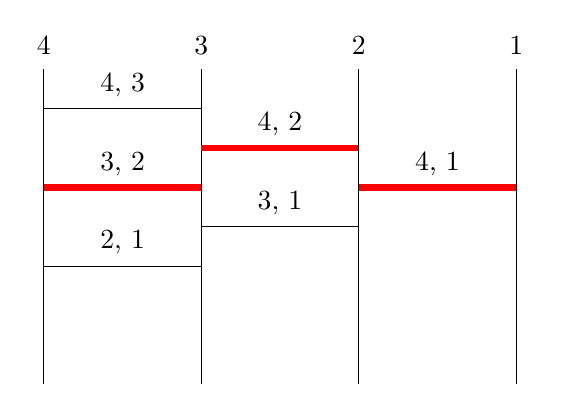
\begin{tikzpicture}
        \draw(0, 0) to (0, 4);
            \node at(0, 4.3){4};
             \draw(0, 3.5) to (2, 3.5);
                \node at(1, 3.8){4, 3};
            
            \draw[line width=0.8mm, red](0, 2.5) to (2, 2.5);
                \node at(1, 2.8){3, 2};

            \draw(0, 1.5) to (2, 1.5);
                \node at(1, 1.8){2, 1};
        \draw(2, 0) to (2, 4);
            \node at(2, 4.3){3};
                \draw[line width=.8mm, red](2, 3) to (4, 3);
                    \node at(3, 3.3){4, 2};
           
                \draw(2, 2) to (4, 2);
                    \node at(3, 2.3){3, 1};
        \draw(4, 0) to (4, 4);
             \node at(4, 4.3){2};
                \draw[line width=0.8mm, red](4, 2.5) to (6, 2.5);
                    \node at (5, 2.8){4, 1};
        \draw(6, 0) to (6, 4);
            \node at(6, 4.3){1};


    \end{tikzpicture}
    \end{center}
    \caption{The root ladder of $(4,3,2,1)$. Note that bar 4,2 is the parent of bar 3,2 and 4,1. Also note that 
    bar 3, 2 is the the left child of 4, 2 and 4, 1 is the right child.}
\end{figure}

The second way to choose the canonical representative is to use a greedy algorithm 
in order to choose the best representative from the next $OptL\{\pi_{N}\}$. 
The is based on comparing the canonical representative from $OptL\{\pi_{i}\}$ with all the ladders in
$OptL\{\pi_{i+1}\}$and choosing the ladder from $OptL\{\pi_{i+1}\}$ that had the least number of 
changes from the canonical ladder from $OptL\{\pi_{i}\}$. Each Gray Code provides a different representative.
Both of the basic operations are used in order to determine the optimal canonical representative.
The canonical representative from $OptL\{\pi_{i+1}\}$ is the ladder with the least number of insertions/deletions 
and least number of swaps when compared to the canonical representative from $OptL\{\pi_{i}\}$.
The canonical representative for $OptL\{\pi_{1}\}$ is the root ladder for the idendity permutation.\par 
In order to see a comparision for the two canonical representative selection methods for permutations of 
size 3 using the modified Zaks algorithm please refer to figure --\pagebreak

\begin{figure}[!htp]
   
 \begin{minipage}{0.1\textwidth}
    \begin{flushleft}
    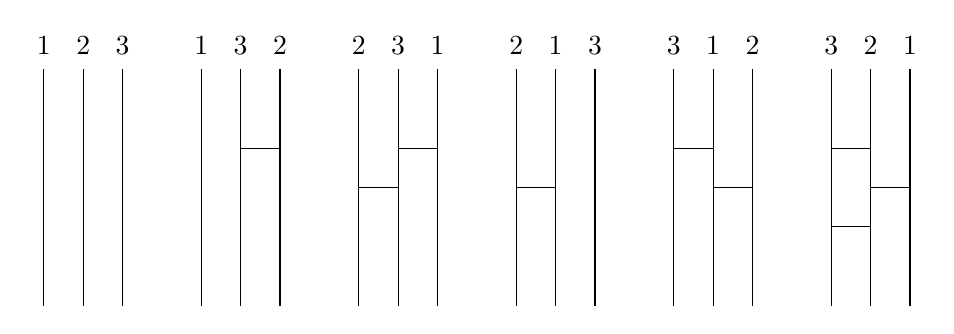
\begin{tikzpicture}

        %%l1
        \draw(0, 0) to (0, 3);
            \node at (0, 3.3){1};
        \draw(0.5, 0) to (0.5, 3);
            \node at (0.5, 3.3){2};
        \draw(1, 0) to (1, 3);
            \node at(1, 3.3){3};

            %%\draw(2.2, 1.5) to (2.8, 1.5);
        %%L2
           \draw(2, 0) to (2, 3);
            \node at (2, 3.3){1};
        \draw(2.5, 0) to (2.5, 3);
            \node at (2.5, 3.3){3};
                \draw(2.5, 2) to (3, 2);
        \draw(3, 0) to (3, 3);
            \node at(3, 3.3){2};

        %%L3
            \draw(4, 0) to (4, 3);
                \node at(4, 3.3){2};
                \draw(4, 1.5) to (4.5, 1.5);
            \draw(4.5, 0) to (4.5, 3);
                \node at(4.5, 3.3){3};
                \draw(4.5, 2) to (5, 2);
            \draw(5, 0) to (5, 3);
                \node at(5, 3.3){1};
        %%L4
            \draw(6, 0) to (6, 3);
                \node at(6, 3.3){2};
                \draw(6, 1.5) to (6.5, 1.5);
            \draw(6.5, 0) to (6.5, 3);
                \node at(6.5, 3.3){1};
            \draw(7, 0) to (7, 3);
                \node at(7, 3.3){3};

         %%L5
            \draw(8, 0) to (8, 3);
                \node at(8, 3.3){3};
                \draw(8, 2) to (8.5, 2);
            \draw(8.5, 0) to (8.5, 3);
                \node at(8.5, 3.3){1};
                \draw(8.5, 1.5) to (9, 1.5);
            \draw(9, 0) to (9, 3);
                \node at(9, 3.3){2};

         %%L6
            \draw(10, 0) to (10, 3);
                \node at(10, 3.3){3};
                \draw(10, 2) to (10.5, 2);
                \draw(10, 1) to (10.5, 1);
            \draw(10.5, 0) to (10.5, 3);
                \node at(10.5, 3.3){2};
                \draw(10.5, 1.5) to (11, 1.5);
            \draw(11, 0) to (11, 3);
                \node at(11, 3.3){1};
    \end{tikzpicture}
\end{flushleft}
\end{minipage}
 

\begin{minipage}{0.1\textwidth}
    \begin{flushleft}
    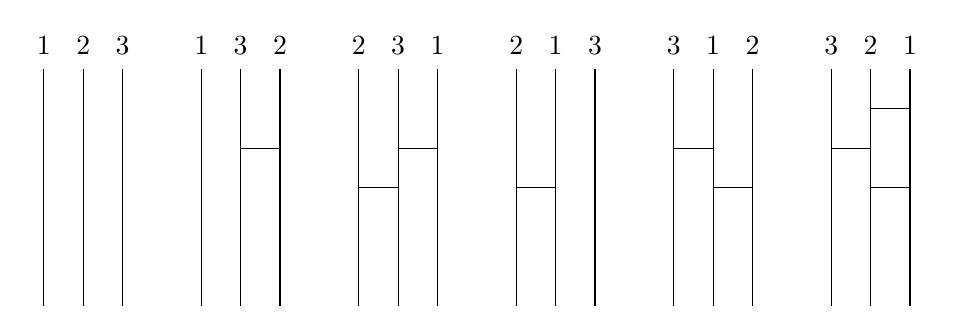
\begin{tikzpicture}

        %%l1
        \draw(0, 0) to (0, 3);
            \node at (0, 3.3){1};
        \draw(0.5, 0) to (0.5, 3);
            \node at (0.5, 3.3){2};
        \draw(1, 0) to (1, 3);
            \node at(1, 3.3){3};

            %%\draw(2.2, 1.5) to (2.8, 1.5);
        %%L2
           \draw(2, 0) to (2, 3);
            \node at (2, 3.3){1};
        \draw(2.5, 0) to (2.5, 3);
            \node at (2.5, 3.3){3};
                \draw(2.5, 2) to (3, 2);
        \draw(3, 0) to (3, 3);
            \node at(3, 3.3){2};

        %%L3
            \draw(4, 0) to (4, 3);
                \node at(4, 3.3){2};
                \draw(4, 1.5) to (4.5, 1.5);
            \draw(4.5, 0) to (4.5, 3);
                \node at(4.5, 3.3){3};
                \draw(4.5, 2) to (5, 2);
            \draw(5, 0) to (5, 3);
                \node at(5, 3.3){1};
        %%L4
            \draw(6, 0) to (6, 3);
                \node at(6, 3.3){2};
                \draw(6, 1.5) to (6.5, 1.5);
            \draw(6.5, 0) to (6.5, 3);
                \node at(6.5, 3.3){1};
            \draw(7, 0) to (7, 3);
                \node at(7, 3.3){3};

         %%L5
            \draw(8, 0) to (8, 3);
                \node at(8, 3.3){3};
                \draw(8, 2) to (8.5, 2);
            \draw(8.5, 0) to (8.5, 3);
                \node at(8.5, 3.3){1};
                \draw(8.5, 1.5) to (9, 1.5);
            \draw(9, 0) to (9, 3);
                \node at(9, 3.3){2};

         %%L6
            \draw(10, 0) to (10, 3);
                \node at(10, 3.3){3};
                \draw(10, 2) to (10.5, 2);
                
            \draw(10.5, 0) to (10.5, 3);
                \node at(10.5, 3.3){2};
                \draw(10.5, 1.5) to (11, 1.5);
                \draw(10.5, 2.5) to (11, 2.5);
            \draw(11, 0) to (11, 3);
                \node at(11, 3.3){1};
    \end{tikzpicture}
\end{flushleft}
\end{minipage}
\caption{The canonical representatives from $N=3$ for all $OptL\{\pi_{3}\}$
using the modified Zaks Gray Code. The top row represents the root ladder as the canonical ladder.
The bottom row represents the greedy choice for the canonical ladder. Notice how the last ladder in the rows 
differ from each other.}
\end{figure}



    

\subsection{Procedure}
Thus far, the problem has been introduced and the basic 
operations have been defined. Recall that there are two basic 
operations; insertion/deletion of a bar or swapping of two bars.
However, there has yet to be discussion regarding the four modified 
Gray Code algorithms used to generate the data. In the procedure section 
we look at the pseudo code for each of the algorithms and explain what 
each of the algorithms are doing. In each of these algorithms, only the root 
ladder is created. The algorithms can be modified by applying  the logic to 
a permutation then calling the enumeration algorithm which will generate $OptL\{\pi_{N}\}$.
This will allow the greedy approach to be applied for selecting the canonical representative.


%%section SJT
\subsubsection{Steinhaus-Johnson-Trotter}\pagebreak


\begin{algorithm}
  \begin{algorithmic}[1]
    \Function{modifiedSjt}{n, ladder, arr, direction}

      %%base case
      \If{$globalCount = n!$}
        \State return
      \EndIf

      %%initial case
      \If{$globalCount = 1$}
        \State $ladder \gets Idendity ladder$
      \EndIf

     
      \State $dir \gets direction[n-1]$

      %%swap the nth element n-1 times
      \For{$i \gets 0$,$i < n-1$, $i \gets i+1$}
        
        \State $arr[n-1] \gets arr[n-1]+1$
        \If{$dir = left$}
          \State add or remove a bar in column to the left
          \Else
            \State add or remove a bar in column to the right
        \EndIf
        \If{$ladder$ has degenerative triadic bar pattern from $basicOpOne$}
          \State swap the bars in the ladder
         \EndIf
        \State $globalCount \gets globalCount+1$

      \EndFor
      \State $direction[n-1] \gets !direction[n-1]$
      \State $HELPERSJT(n-1, ladder, arr, direction)$
      \State $MODIFIEDSJT(n,  ladder, arr, direction)$

    \EndFunction
  \end{algorithmic}
\end{algorithm}

%%helper algorithm
\begin{algorithm}
  \begin{algorithmic}[1]
    \Function{helpersjt}{n, ladder, arr, direction}
      \For{$i \gets n-1$, $i \geq 0$, $i\ gets i-1$}
        \If{$arr[i] < i$}
          \If{$dir[i] = LEFT$}
            \State add or remove a bar in column to the left 
          \Else
            \State add or remove a bar in column to the right
          \EndIf
          \State $arr[i]\gets arr[i+1]$
          \State return
        \Else 
          \State $arr[i] \gets 0$
          \State $direction[i] \gets !direction[i]$
        \EndIf
      \EndFor
      \EndFunction
  \end{algorithmic}
\end{algorithm}

The principles that act as the foundation for the modified SJT algorithm following. $N$ represents the length of the array that the ladder 
corresponds to. $arr$ represents the elements from $1$ to $N-1$ and is 
used to keep track of how many times a bar corresponding to one of their routes 
has been added or removed. $dir$ represents the current direction for 
each element from $1 \dots N$. The direction is switched when each element has had a 
bar added or removed from its route $N-1$ times going in one direction. 
Insert or remove a bar belonging to the route of the $Nth$ element going 
from left to right or right to left. Once the first or last column has had a bar 
belonging to the $Nth$ element added or removed, switch the direction for the $Nth$
element then remove or add a bar corresponding to the 
$N-Rth$ element where $R>1$. It is this stage in which $HELPERSJT$ is called. When a bar 
is added or removed from the $N-Rth$ element, the array at the position representing 
that element is increased by one. If the array at that index representing the element 
equals $N-R$ then reset it to zero and move onto the next element less than $N-R$. This step can be found 
on line(s) 3 and 10 in $HELPERSJT$. Once the $N-Rth$ element has had a bar added or removed from the first or last column, 
continue with $MODIFIEDSJT$ until $globalCount=n!$. The algorithm requires $O(1)$ time for the insertion or 
deletion of a bar. The procedure is done $n!$ times. Swapping two bars takes $O(1)$ time. The procedure is done 
$(n-1)!$ times.\pagebreak



%%Section: Heaps
\subsubsection{Heap's Algorithm}

\begin{algorithm}
  \begin{algorithmic}[1]
    \Function{modifiedHeaps}{Ladder, index, permuation}
      \If{$index=0$}
        \State return
      \EndIf
      \For{$i\gets 0, i<index, i\gets i+1$}
        
        $MODIFIEDHEAPS(Ladder, index-1)$
        \If{$index$ is even}
          \State $swap(perm[0], perm[index])$
        \Else 
          \State $swap(perm[i], perm[index])$
          
        \EndIf
        \State $Ladder \gets Root_{permuation}$
      \EndFor
      \If{$index > 1$}
        \State $MODIFIEDHEAPS(Ladder, index-1)$
      \EndIf
    \EndFunction
  \end{algorithmic}
\end{algorithm}
The principles that act as the foundation for the modified Heap's algorithm 
are the following. Initially begin with the Idendity ladder, when the index is 
even insert swap the element in $\pi$ at zero with the element and index-1. Then create the 
corresponding root ladder. Otherwise swap the value at the counter with the value at the 
index and create the corresponding root ladder. The time complexity for swapping two elements 
is $O(1)$. This is done $n!$ times. Add this to the cost of creating the root ladder which is 
$n^{3}$.\pagebreak



%%Section Zaks
\subsubsection{Zaks Algorithm}
%%main driver
\begin{algorithm}
  \begin{algorithmic}[1]
    \Function{modifiedZaks}{permutation, ladder, suffixVector, n, index}
      \If{$GlobalCount = n!$}
        \State return
      \EndIf
        \State $endIndx \gets n-1$
        \State $startIndx \gets n-suffixVector[index]$
        \State reverse $permutation's$ suffix starting from $startIndx$ to $endIndx$
        \State $ladder \gets Root_{permutation}$.
        \State $index \gets index+1$
        \State$MODIFIEDZAKS(permutation, ladder, suffixVector, n, index+1)$ 


    \EndFunction
  
  
  \end{algorithmic}

\end{algorithm}


%%helpe function
\begin{algorithm}
  \begin{algorithmic}[1]
    \Function{createsuffix}{suffixVector, n}
      \If{$n = 2$}
        \State append 2 to $suffixVector$
        \State return
      \EndIf

        $CREATESUFFIX(suffixVector, n-1)$
        
        $temp \gets$ suffixVector
        \For{$i \gets 0$, $i < n-1$, $i \gets i+1$}

          \State append $n$ to $suffixVector$
          \State append $temp$ to $suffixVector$
        \EndFor
    \EndFunction
  \end{algorithmic}
\end{algorithm}\pagebreak

The principles that act as the foundation for the modified Zaks 
algorithm are the following. First, the suffix vector is created. 
The suffix vector is created with the following recurrence relation.
\begin{center}
  $S_{2} = 2$\newline
  $S_{N} = (S_{N-1},N)^{n-1}N-1, n>2$\newline
\end{center}

\begin{example}
  \begin{center}


  $N=2$\newline
  $S_{2} = 2$\newline
  $(1,2), (2,1)$\newline

  $N=3$\newline
  $S_{3} = 23232$\newline 
  $(1,2,3), (1,3,2), (2,3,1), (2,1,3), (3,1,2), (3,2,1)$\newline
  \end{center}
\end{example}
The suffix vector represents the suffix of the permutation that is to 
be reversed. The procedure begings with the Idendity permuation of 
size $N$. If $N$ is $2$ then reverse the only two elements in $\pi$.
Else reverse the suffix of size $N-1$ $(N-1)!$ times, with $1$ being unmoved.
Then reverse the entire permutation, putting element $1$ at the end of the permuation.
Repeat these steps, now with element $2$ as the prefix, thus leaving element 
$2$ unmoved for the next round of $(N-1)!$ reversals. Repeat the process 
$N!$ which results in the reverse permuation.\par 
Once the suffix vector is created, on each call to the main function, use 
the current value of the suffix vector to indicate the size of the suffix to 
reverse, then reverse said suffix in the permutation and create the corresponding root ladder 
from the resulting permutation Reversing a suffix takes $O(N)$ time. This is done $N!$ times.
The cost of creating the root ladder is $O(N^{3})$.



%%Section Lex
\subsubsection{Lexicographic Algorithm}

\begin{algorithm}
  \begin{algorithmic}[1]
    \Function{modifiedlex}{perm, ladder, n}
      \If{$globalCount = n!$}
        \State return
      \EndIf
      \For{$i \gets n-1$, $i > 0$, $i \gets i-1$}
        \If{$perm[i-1]<perm[i]$}
          \State $maxMin \gets $ min value $>$ $perm[i-1]$ and to the right of 
          $perm[i-1]$
          
                                  
          \State $swap(perm[i-1], maxMin)$
          \State sort $perm$ from index $i$ to index $n-1$ in ascending order
          \State $ladder \gets Root_{perm}$
          \State $MODIFIEDLEX(perm, ladder, n)$
        \EndIf
      \EndFor

    \EndFunction
  \end{algorithmic}
\end{algorithm}

The principles founding the modified lexicographic algorithm are the following.
On each call to the algorithm, begin at the end of the permutation and 
find a decreasing subsequence going right to left. Once found, get the index 
of the lesser element. Then go to the right of the lesser element and find the 
smallest value greater than the lesser element. Swap this element with the lesser element. 
Sort the section of the array that is to the right of the original index of the 
lesser element before it was swapped. Once sorted, create the root ladder corresponding 
to this new permutation. The cost of sorting a suffix is $Nlog{N}$ and is done $N!$ times.
The cost of creating the root ladder is $N^{3}$.

\subsubsection{Algorithmic Analysis}
  It should be noted that only the modified SJT algorithm has been customized for ladder lotteries. The rest of the algorithms 
  require a permutation in order to generate the corresponding root ladder from the permutation. More work needs to be done in 
  order to create the proper modified Gray Code algorithms customized for ladder-lotteries. 
  Nonetheless, the above algorithms allow for analysis of the two basic operations which in turn can lead to determining which Gray Code is best 
  for enumerating the canonical representative. These results will be discussed in the next section.
\subsection{Results}

The results for the two basic operations are listed in the tables below. There are two separate tables, one 
for the root ladder as the canonical representative, the other for the optimal ladder as the canonical representative.
The results for $N=6$ are listed. The average number of swaps and the average number of insertions or deletions are 
recorded for each algorithm.

%%first table
\begin{tabular}{ |p{3cm}||p{3cm}|p{3cm}|p{3cm}}
 \hline
 \multicolumn{4}{|c|}{Root Ladder} \\
 \hline
 Gray Code& Operatin One &Operation Two& N\\
 \hline
 SJT  & 1.000000 &0.200000 & 3\\
 HEAPS & 1.800000 & 0.000000 & 3 \\
 ZAKS & 1.8000000 & 0.2000000 &  3\\
 LEX & 1.400000 & 0.2000000 &  3\\

 SJT  & 1.000000 &0.200000 & 3\\
 HEAPS & 1.800000 & 0.000000 & 3 \\
 ZAKS & 1.8000000 & 0.2000000 &  3\\
 LEX & 1.400000 & 0.2000000 &  3\\
 
 SJT  & 1.000000 &0.200000 & 3\\
 HEAPS & 1.800000 & 0.000000 & 3 \\
 ZAKS & 1.8000000 & 0.2000000 &  3\\
 LEX & 1.400000 & 0.2000000 &  3\\
 
 SJT  & 1.000000 &0.200000 & 3\\
 HEAPS & 1.800000 & 0.000000 & 3 \\
 ZAKS & 1.8000000 & 0.2000000 &  3\\
 LEX & 1.400000 & 0.2000000 &  3\\
 \hline
\end{tabular}



%----------------  EVALUATION or ANALYSIS ------------------------------------------
\chapter{Evaluation}  
\label{chapter:evaluation}


%----------------  SUMMARY AND FUTURE WORK -----------------------------------

\chapter{Summary and Future Work}
\label{chapter:summary}

Conclude your thesis with a re-cap of your major results and contributions.  Then outline directions for further research and remaining open problems.

%--- BIBLIOGRAPHY  ------
\ssp
  \bibliographystyle{abbrv}
  \bibliography{mybib}
\dsp

%--- APPENDIX  ------

\appendix
\include{Appendix}

\end{document} 